% Copyright 2004 by Till Tantau <tantau@users.sourceforge.net>.
%
% In principle, this file can be redistributed and/or modified under
% the terms of the GNU Public License, version 2.
%
% However, this file is supposed to be a template to be modified
% for your own needs. For this reason, if you use this file as a
% template and not specifically distribute it as part of a another
% package/program, I grant the extra permission to freely copy and
% modify this file as you see fit and even to delete this copyright
% notice. 

\documentclass{beamer}
% There are many different themes available for Beamer. A comprehensive
% list with examples is given here:
% http://deic.uab.es/~iblanes/beamer_gallery/index_by_theme.html
% You can uncomment the themes below if you would like to use a different
% one:
%\usetheme{AnnArbor}
%\usetheme{Antibes}
%\usetheme{Bergen}
%\usetheme{Berkeley}
%\usetheme{Berlin}
%\usetheme{Boadilla}
%\usetheme{boxes}
%\usetheme{CambridgeUS}
%\usetheme{Copenhagen}
%\usetheme{Darmstadt}
%\usetheme{default}
%\usetheme{Frankfurt}
%\usetheme{Goettingen}
%\usetheme{Hannover}
%\usetheme{Ilmenau}
%\usetheme{JuanLesPins}
%\usetheme{Luebeck}
\usetheme{Madrid}
%\usetheme{Malmoe}
%\usetheme{Marburg}
%\usetheme{Montpellier}
%\usetheme{PaloAlto}
%\usetheme{Pittsburgh}
%\usetheme{Rochester}
%\usetheme{Singapore}
%\usetheme{Szeged}
%\usetheme{Warsaw}

\usepackage{multimedia}
\usepackage{subfig}
%\usebackgroundtemplate{\includegraphics[width= \paperwidth, height=\paperheight]{imagen2}}
\setbeamertemplate{footline}{} 
\title{Sistema de control autónomo en FPGAs libres para robots}

% A subtitle is optional and this may be deleted
\subtitle{}

\author{Juan Ordóñez Cerezo\inst{1}}
% - Give the names in the same order as the appear in the paper.
% - Use the \inst{?} command only if the authors have different
%   affiliation.

\institute[Universidad de Granada] % (optional, but mostly needed)
{
  \inst{1}%
  Universidad de Granada
}
% - Use the \inst command only if there are several affiliations.
% - Keep it simple, no one is interested in your street address.

\date{}
% - Either use conference name or its abbreviation.
% - Not really informative to the audience, more for people (including
%   yourself) who are reading the slides online

\subject{}
% This is only inserted into the PDF information catalog. Can be left
% out. 

% If you have a file called "university-logo-filename.xxx", where xxx
% is a graphic format that can be processed by latex or pdflatex,
% resp., then you can add a logo as follows:

% \pgfdeclareimage[height=0.5cm]{university-logo}{university-logo-filename}
% \logo{\pgfuseimage{university-logo}}

% Delete this, if you do not want the table of contents to pop up at
% the beginning of each subsection:
\AtBeginSubsection[]
{
  \begin{frame}<beamer>{Outline}
    \tableofcontents[currentsection,currentsubsection]
  \end{frame}
}

% Let's get started
\begin{document}

\begin{frame}
  \begin{center}
  
\includegraphics [width =0.5\textwidth ]{logo_ugr}
  \end{center}
    \begin{center}
	
\includegraphics [width =0.4\textwidth ]{logo_rey}
	\end{center}
  \titlepage
\end{frame}

\begin{frame}{Index}
  \tableofcontents
  % You might wish to add the option [pausesections]
\end{frame}

\section{Contexto}
%%%%%%%%%%%%%%%%%%%%%%%%%%%%%%%%%%%%%%%%%%%%%%%%%%%%%%%%%%%%%%%%%%%%%%%%%%%%%%%

\begin{frame}{Contexto}
\begin{block}{}
	\centering	\textbf{Robots Autónomos}
\end{block}
\begin{figure}[H]
	\center	
	\subfloat[Roomba]{
		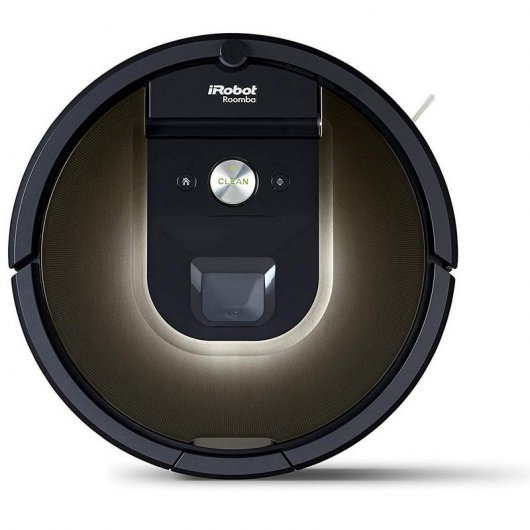
\includegraphics[trim = 0mm 0mm 0mm 0mm, clip,scale=0.25]{imagenes/Introduction/roomba}}
	\subfloat[Boston dynamics]{
		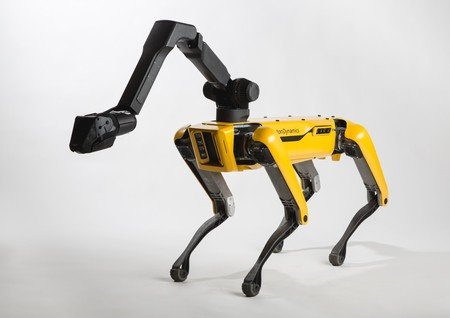
\includegraphics[trim = 0mm 0mm 0mm 0mm, clip,scale=0.35]{imagenes/Introduction/boston}}
\end{figure}
\end{frame}

\begin{frame}{Contexto}
\begin{block}{}
	\centering	\textbf{Robótica Educativa}
\end{block}
		\begin{figure}[H]
	\center
	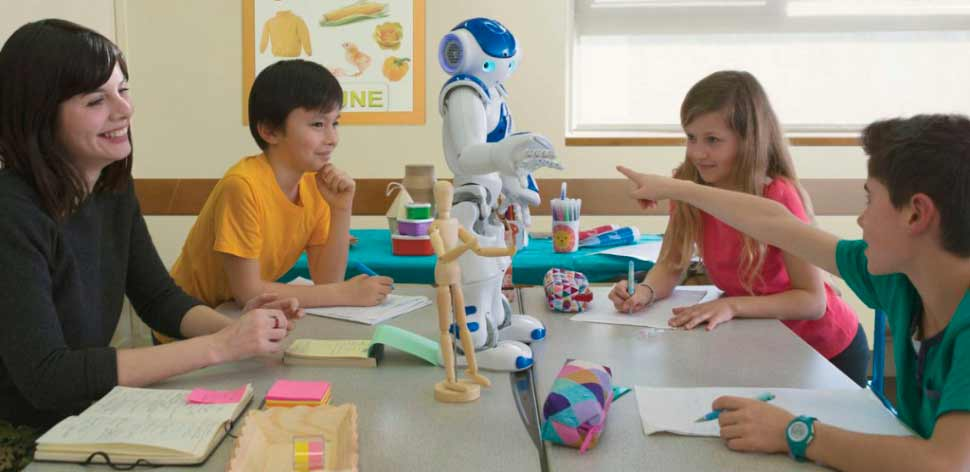
\includegraphics[trim = 0cm 0mm 0mm 0cm,clip, angle=0, scale = 0.3]{imagenes/Introduction/robotica}
\end{figure}
\end{frame}

\section{Infraestructura}
\begin{frame}{IceStudio}
		\begin{figure}[H]
	\center
	
\includegraphics[trim = 0cm 0mm 0mm 0cm,clip, angle=0, scale = 0.3]{imagenes/Introduction/IceStudio}
\end{figure}
	\begin{block}{}
		\begin{itemize}
			\item En este contexto nace IceStudio \pause
			\item Ensalza el uso de FPGAs inlcuyendo todas sus ventajas \pause
			\item Permite implementación hardware de manera gráfica \pause
			\item Ventaja: Configuración del nivel de abstracción 
		\end{itemize}
	\end{block}
\end{frame}

\begin{frame}{IceStudio}
	\begin{figure}[H]
		\center
		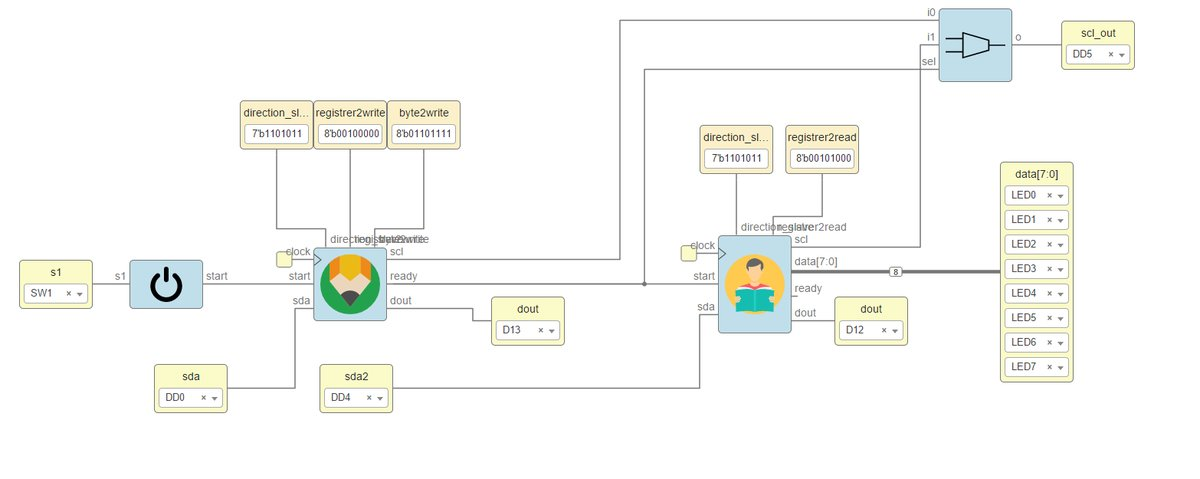
\includegraphics[trim = 0cm 0mm 0mm 0cm,clip, angle=0, scale = 0.3]{imagenes/Introduction/i2creadandwrite}
	\end{figure}
\end{frame}

\begin{frame}{IceStudio}
\begin{figure}[H]
	\center
	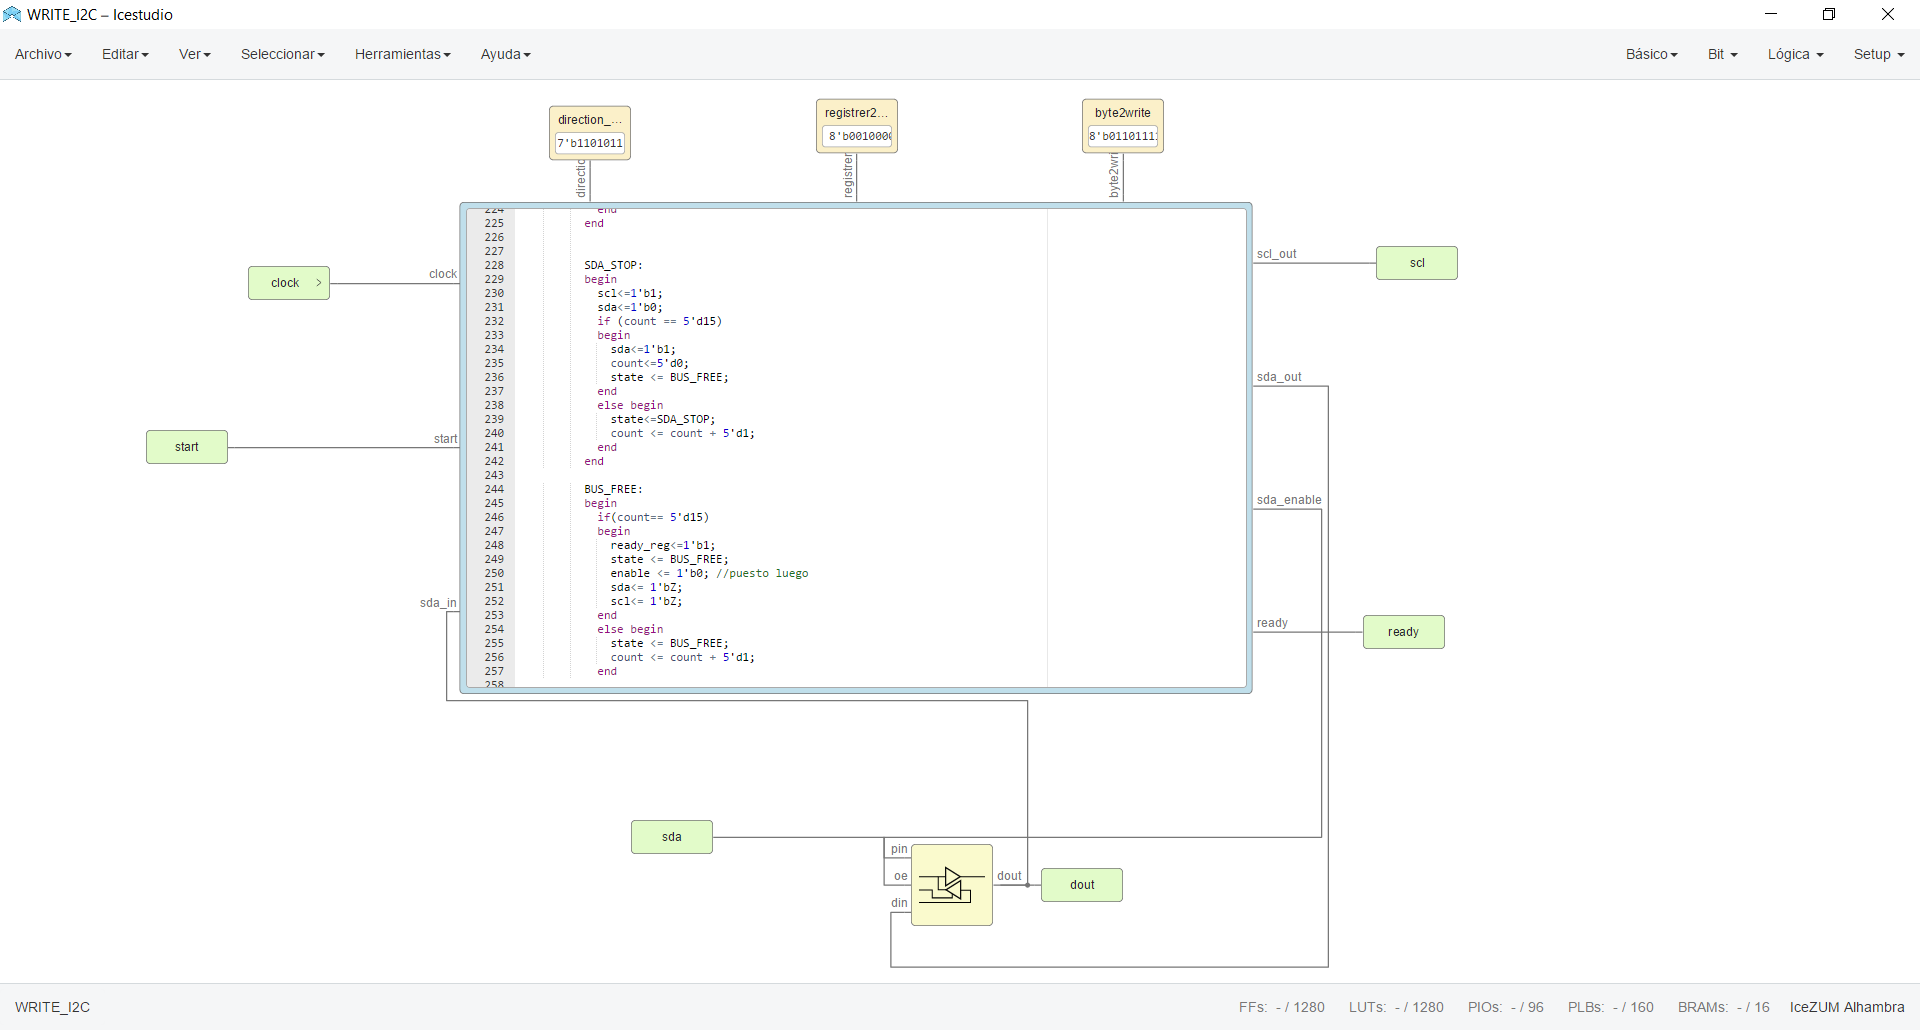
\includegraphics[trim = 0cm 0mm 0mm 0cm,clip, angle=0, scale = 0.3]{imagenes/Introduction/IceStudioI2c}
\end{figure}
\end{frame}

\begin{frame}{IceZum Alhambra}
	\begin{block}{}
		\begin{itemize}
			\item Tarjeta FPGA con Lattice iCE40HK \pause
			\item 4K de memoria \pause
			\item 12 pines digitales \pause
			\item 3 pines analógicos mediante i2c \pause
		\end{itemize}
	\end{block}
\begin{alertblock}{}
		\centering	\textbf{Diseñada y ensamblada en Granada}
		\begin{figure}[H]
			\center
			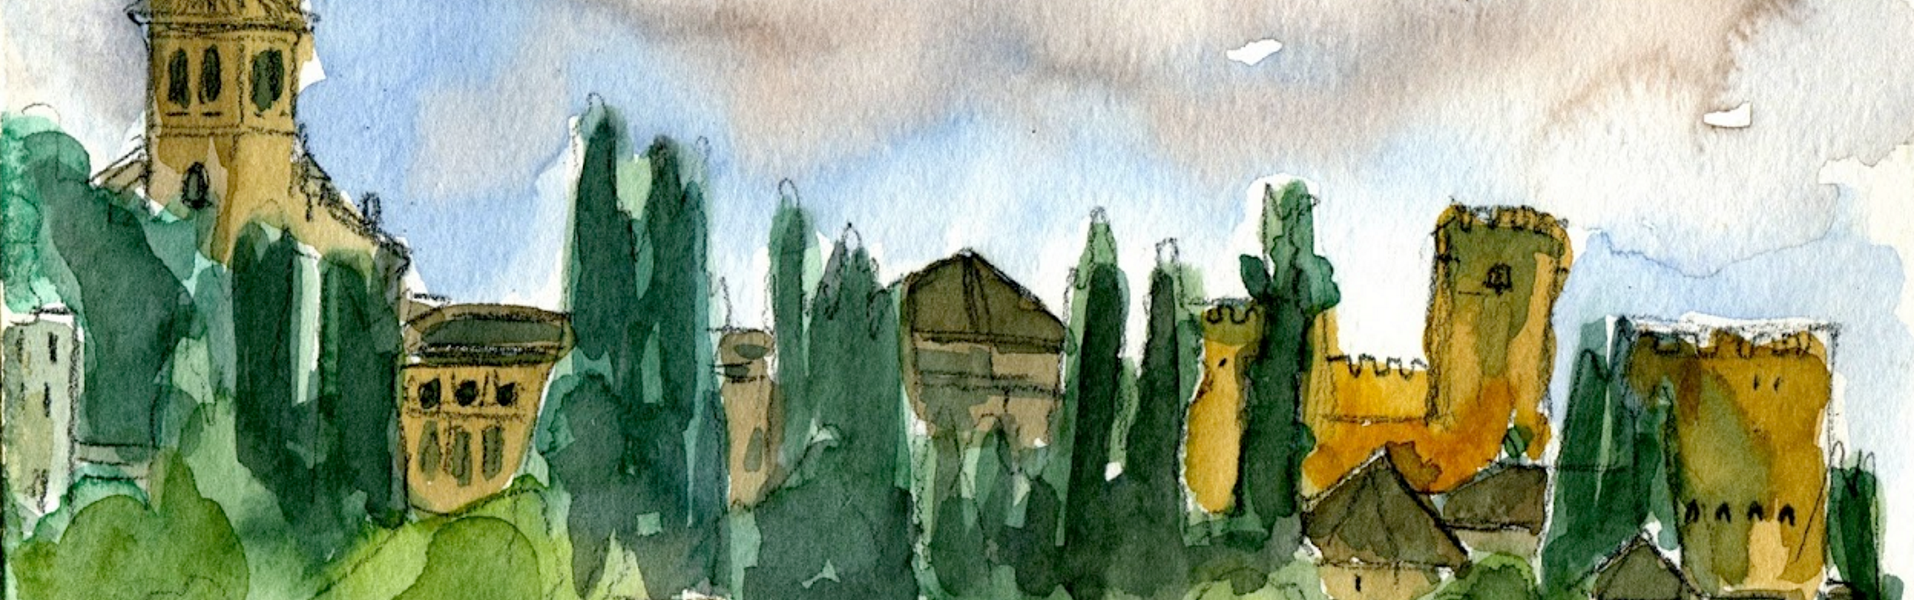
\includegraphics[trim = 0cm 0mm 0mm 0cm,clip, angle=0, scale = 0.2]{imagenes/Introduction/alhambrabits}
		\end{figure}
\end{alertblock}
\end{frame}

\begin{frame}{IceZum Alhambra}
	\begin{figure}[H]
		\center
		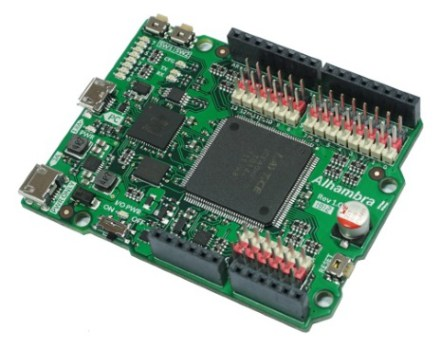
\includegraphics[trim = 0cm 0mm 0mm 0cm,clip, angle=0, scale = 0.5]{imagenes/EstadoArte/IceZumAlhambraII}
	\end{figure}
\end{frame}

\begin{frame}{Planificación y Metodología de trabajo}
	\begin{center}
		\begin{figure}[H]
			\center
			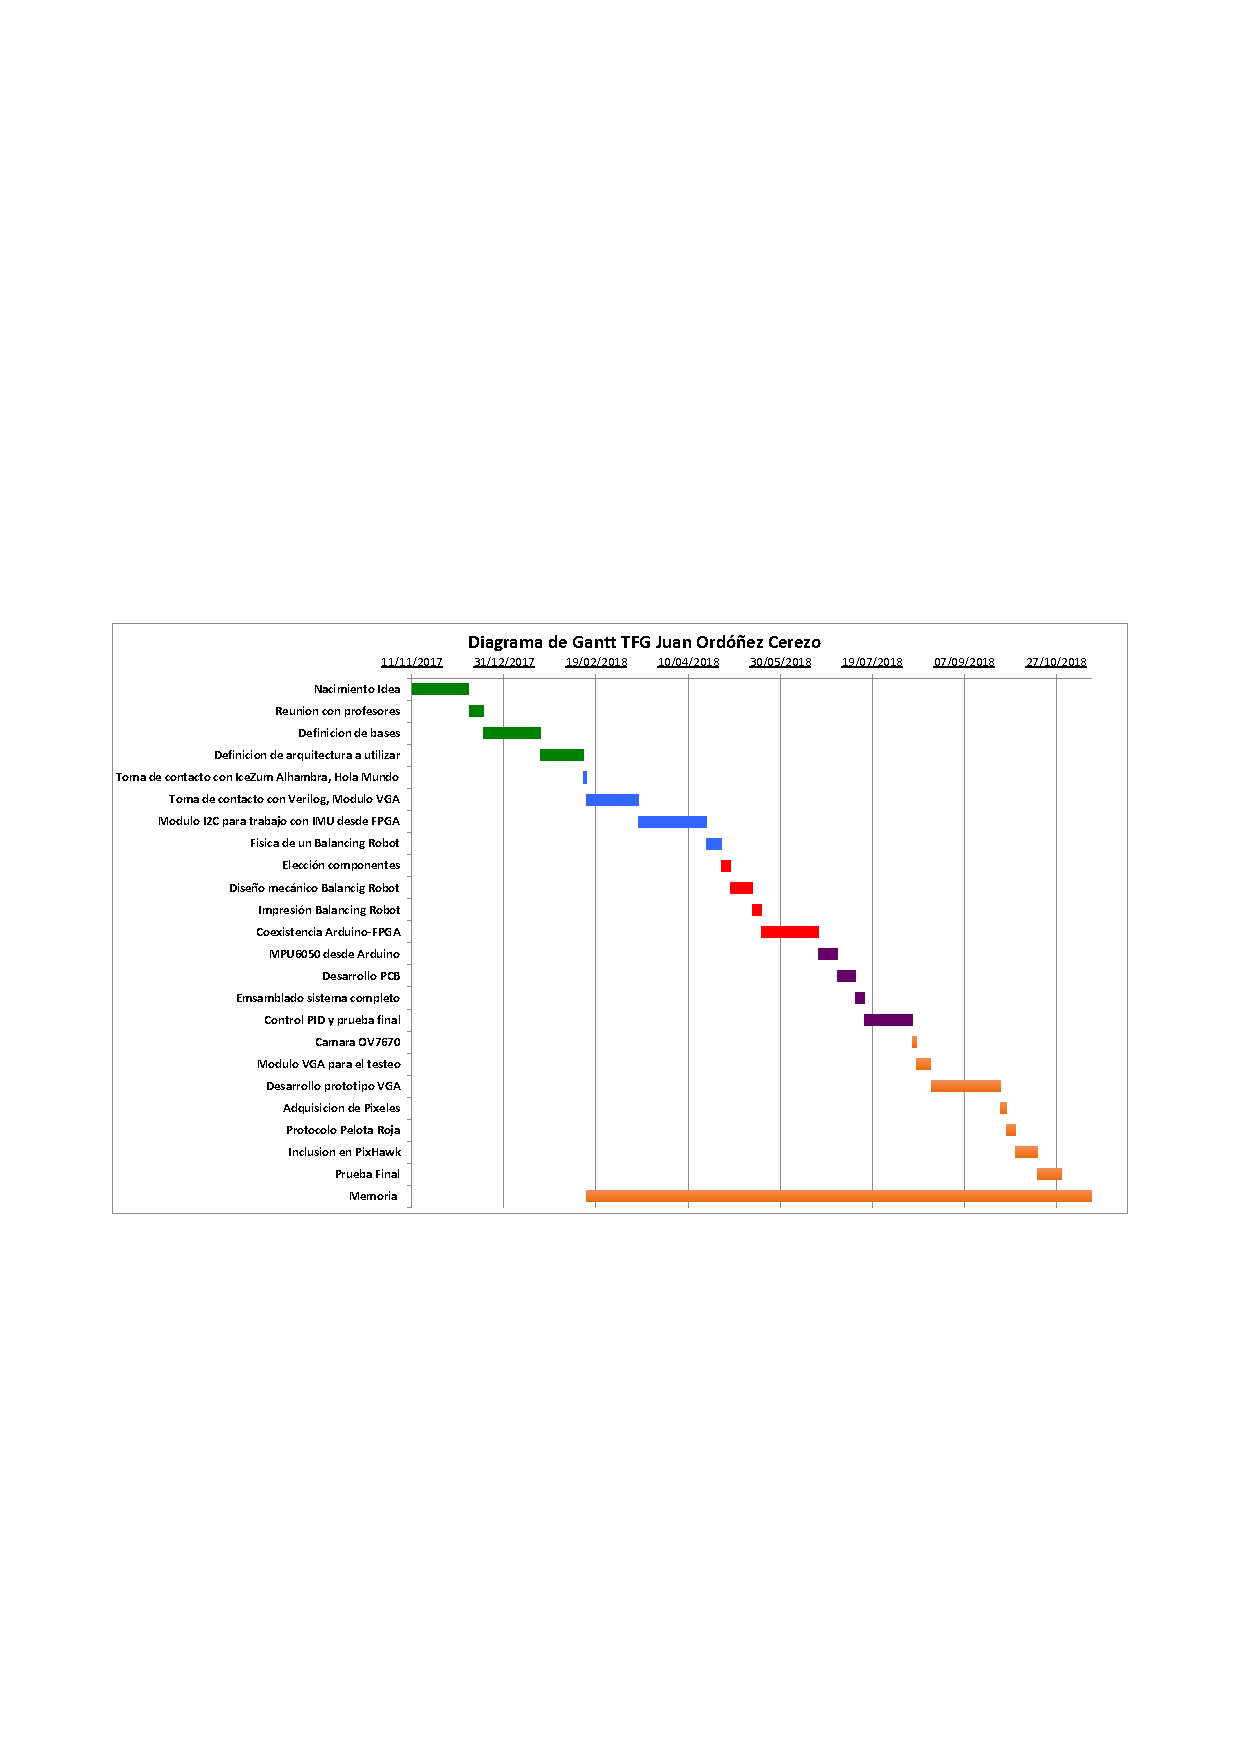
\includegraphics[trim = 1.3cm 0mm 0mm 10.5cm,clip, angle=0, scale = 0.65]{imagenes/Introduction/Gantt.pdf}

		\end{figure}
	\end{center}
\end{frame}

\begin{frame}{Planificación y Metodología de trabajo}
\begin{figure}[H]
	\center	
	\subfloat[GitHub]{
	
\includegraphics[trim = 0mm 0mm 0mm 0mm, clip,scale=0.3]{imagenes/Introduction/github}}
	\subfloat[Appear]{
	
\includegraphics[trim = 0mm 0mm 0mm 0mm, clip,scale=0.2]{imagenes/Introduction/appear}}
\end{figure}
\end{frame}

\section{Objetivos}
\begin{frame}{Objetivos}
\begin{block}{}
	\begin{itemize}
		\item Comportamientos robóticos mediante lenguajes de implementación hardware \pause
		\item Uso de herramientas libres como IceStudio o IceZum Alhambra \pause
		\item Habilidad para el desarrolla de PCB \pause
		\item Habilidad para el diseño e impresión de estrucuturas mecánicas \pause
		\item Entender la importancia de la coexistencia entre microcontrolador y FPGA 
	\end{itemize}
\end{block}
\end{frame}

%%%%%%%%%%%%%%%%%%%%%%%%%%%%%%%%%%%%%%%%%%%%%%%%%%%%%%%%%%%%%%%%%%%%
\section{Robot Balancín}
\subsection{Diseño del sistema}
\begin{frame}{Diseño del sistema}
\begin{figure}[H]
	\center
	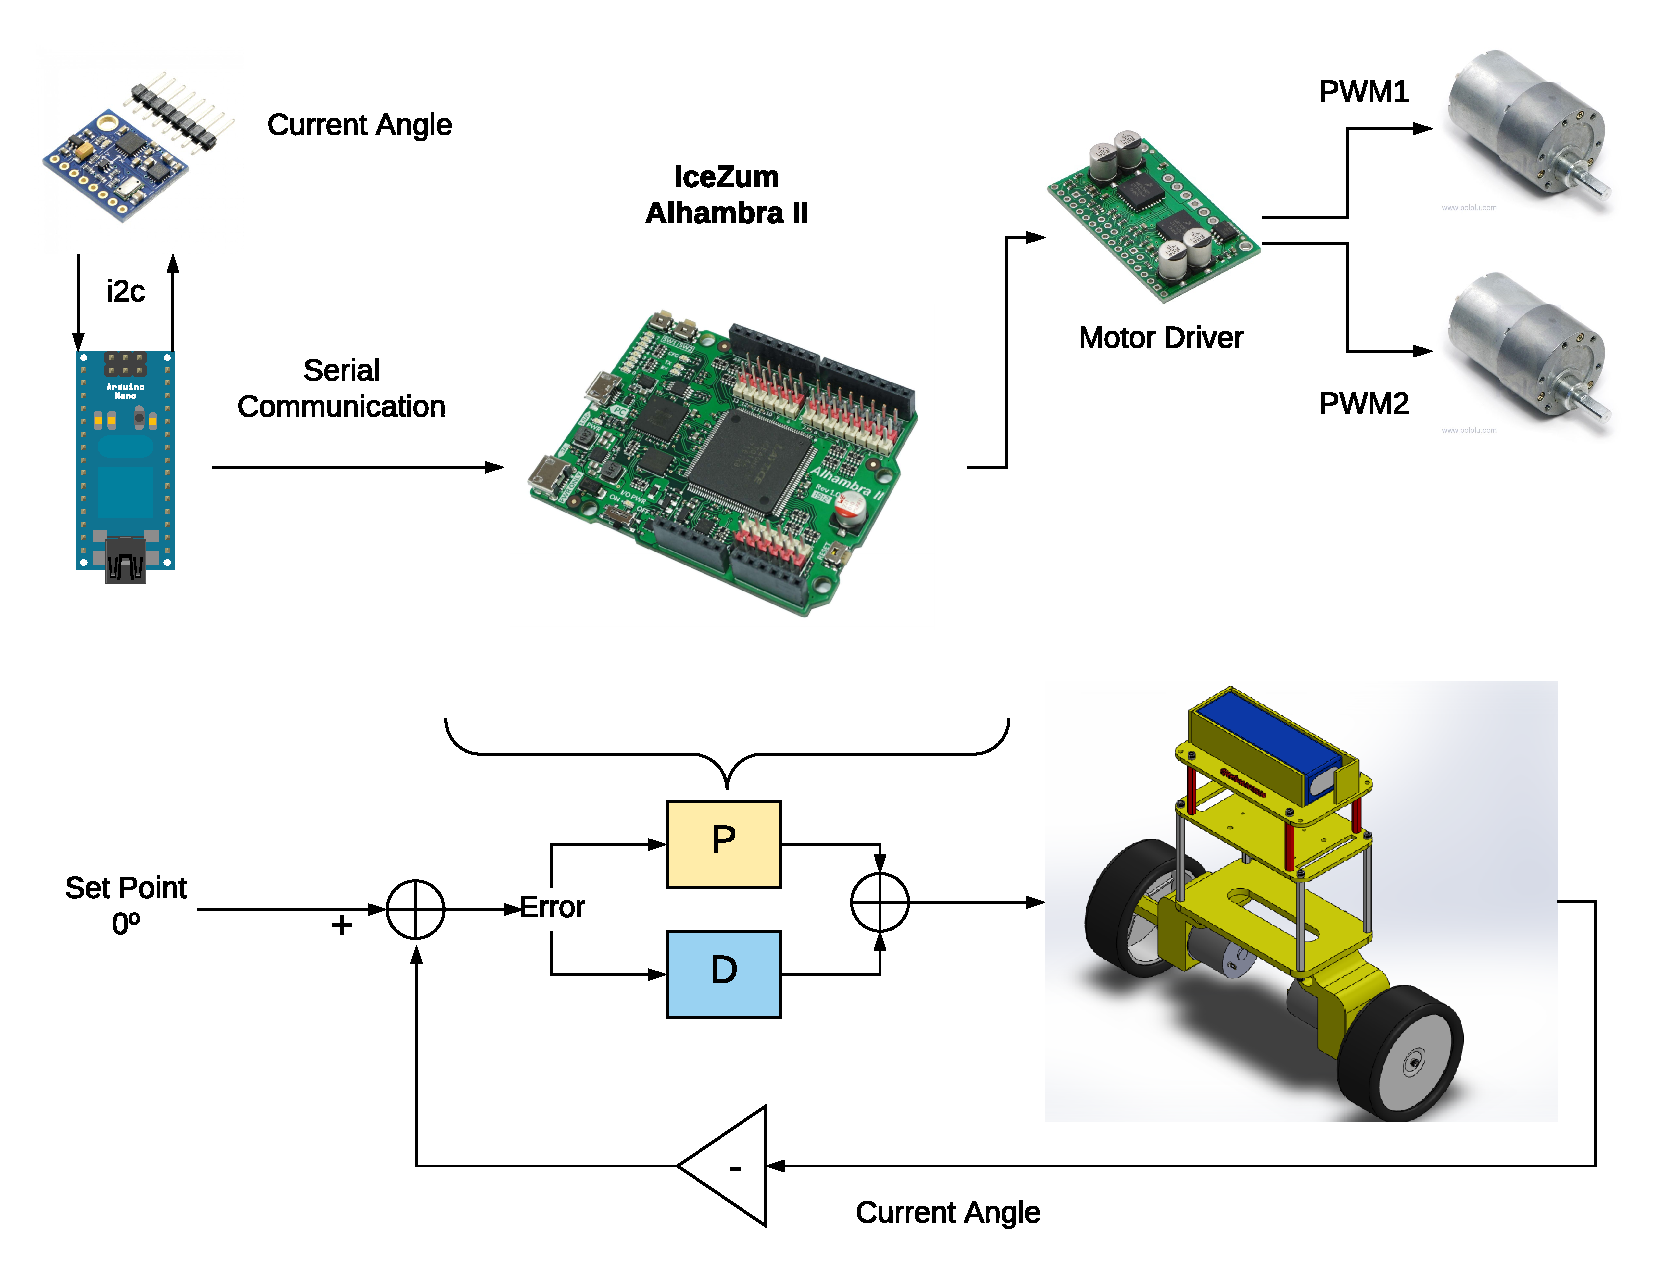
\includegraphics[trim = 0mm 0mm 0mm 0mm, clip,scale=0.3]{imagenes/Balancing_robot/final.pdf}
	\caption{}
	\label{}
\end{figure}
\end{frame}	
\subsection{Implementación del sistema}

\begin{frame}{Estructura mecánica}
\begin{center}
	\begin{figure}[H]
		\center
		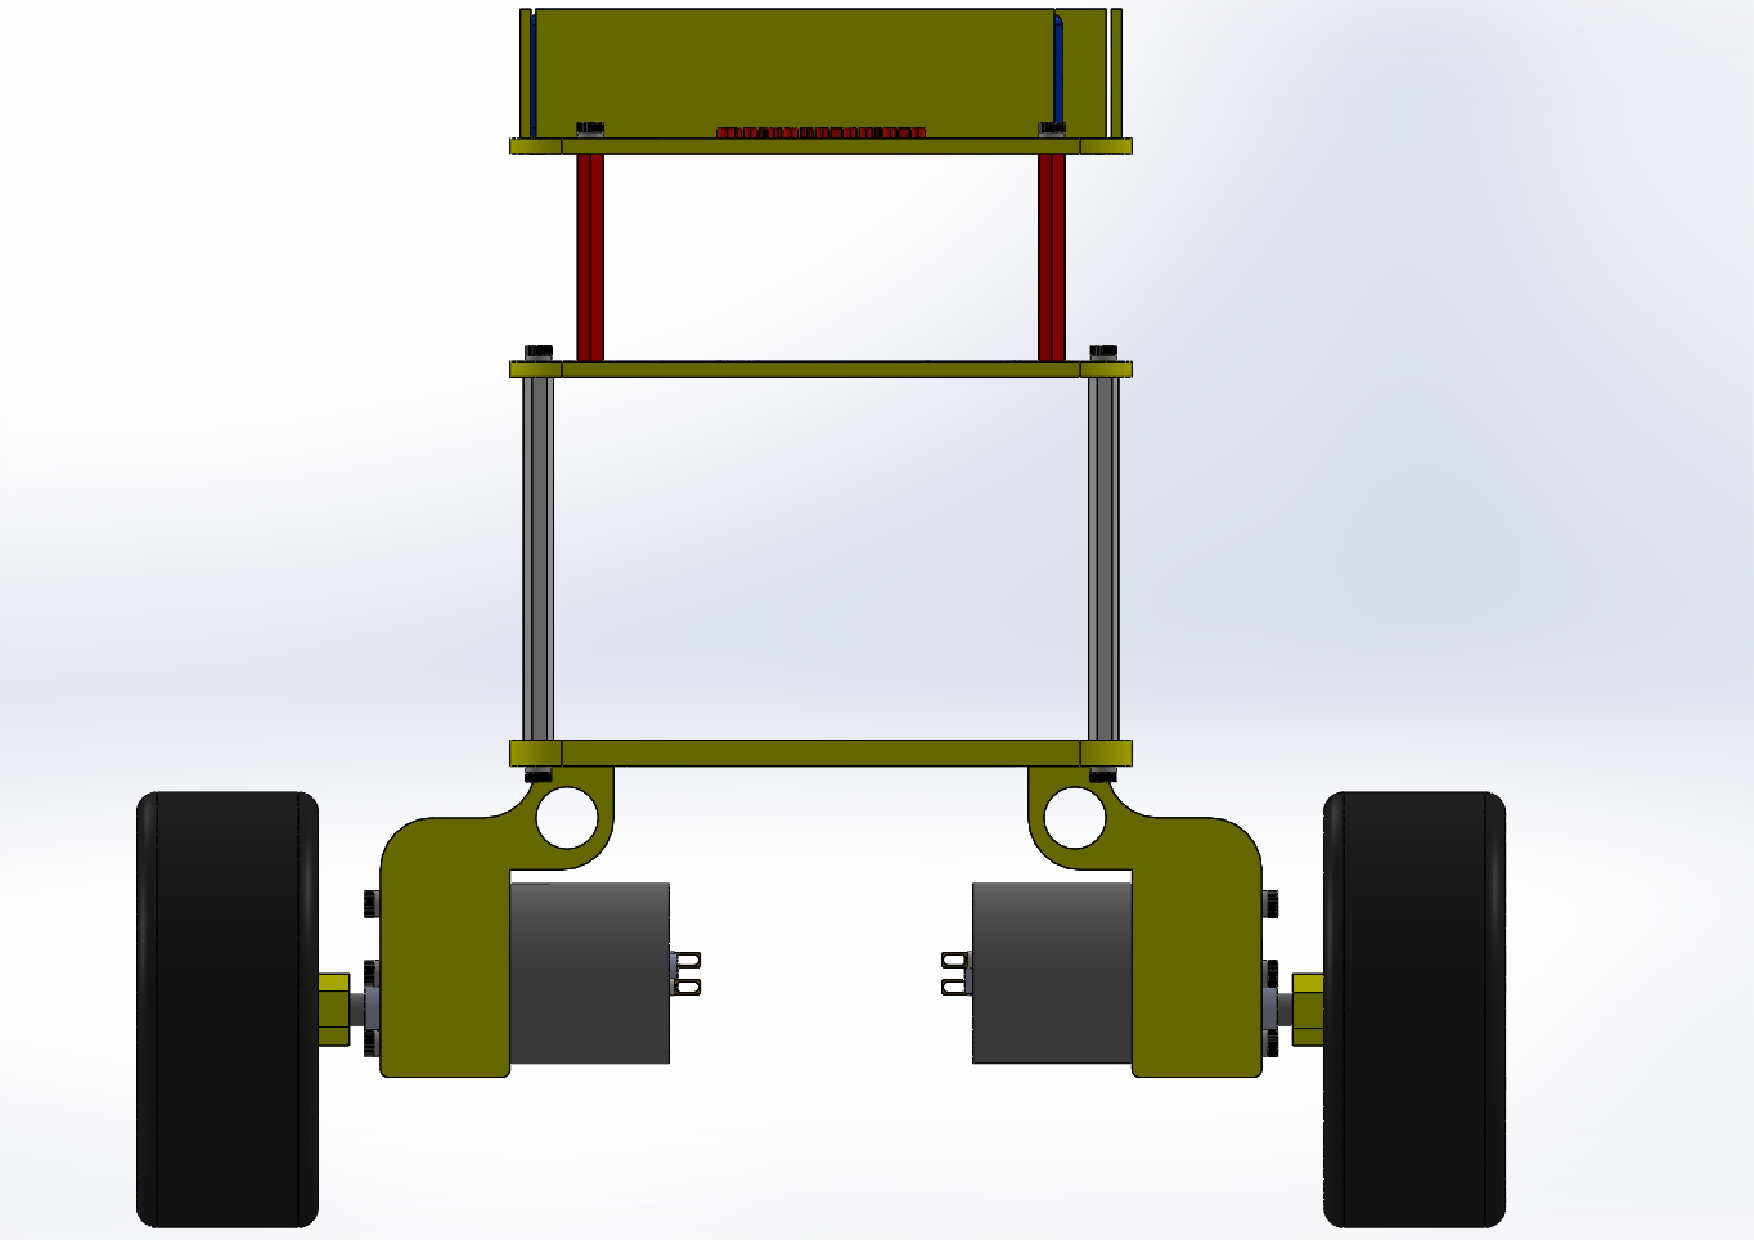
\includegraphics[trim = 1cm 0mm 2.7cm 0mm,clip, angle=0, scale = 0.35]{imagenes/Balancing_Robot/EnsanBalanceFront.PDF}
	\end{figure}
\end{center}
\end{frame}

\begin{frame}{Estructura mecánica}
\begin{center}
	\begin{figure}[H]
		\center
		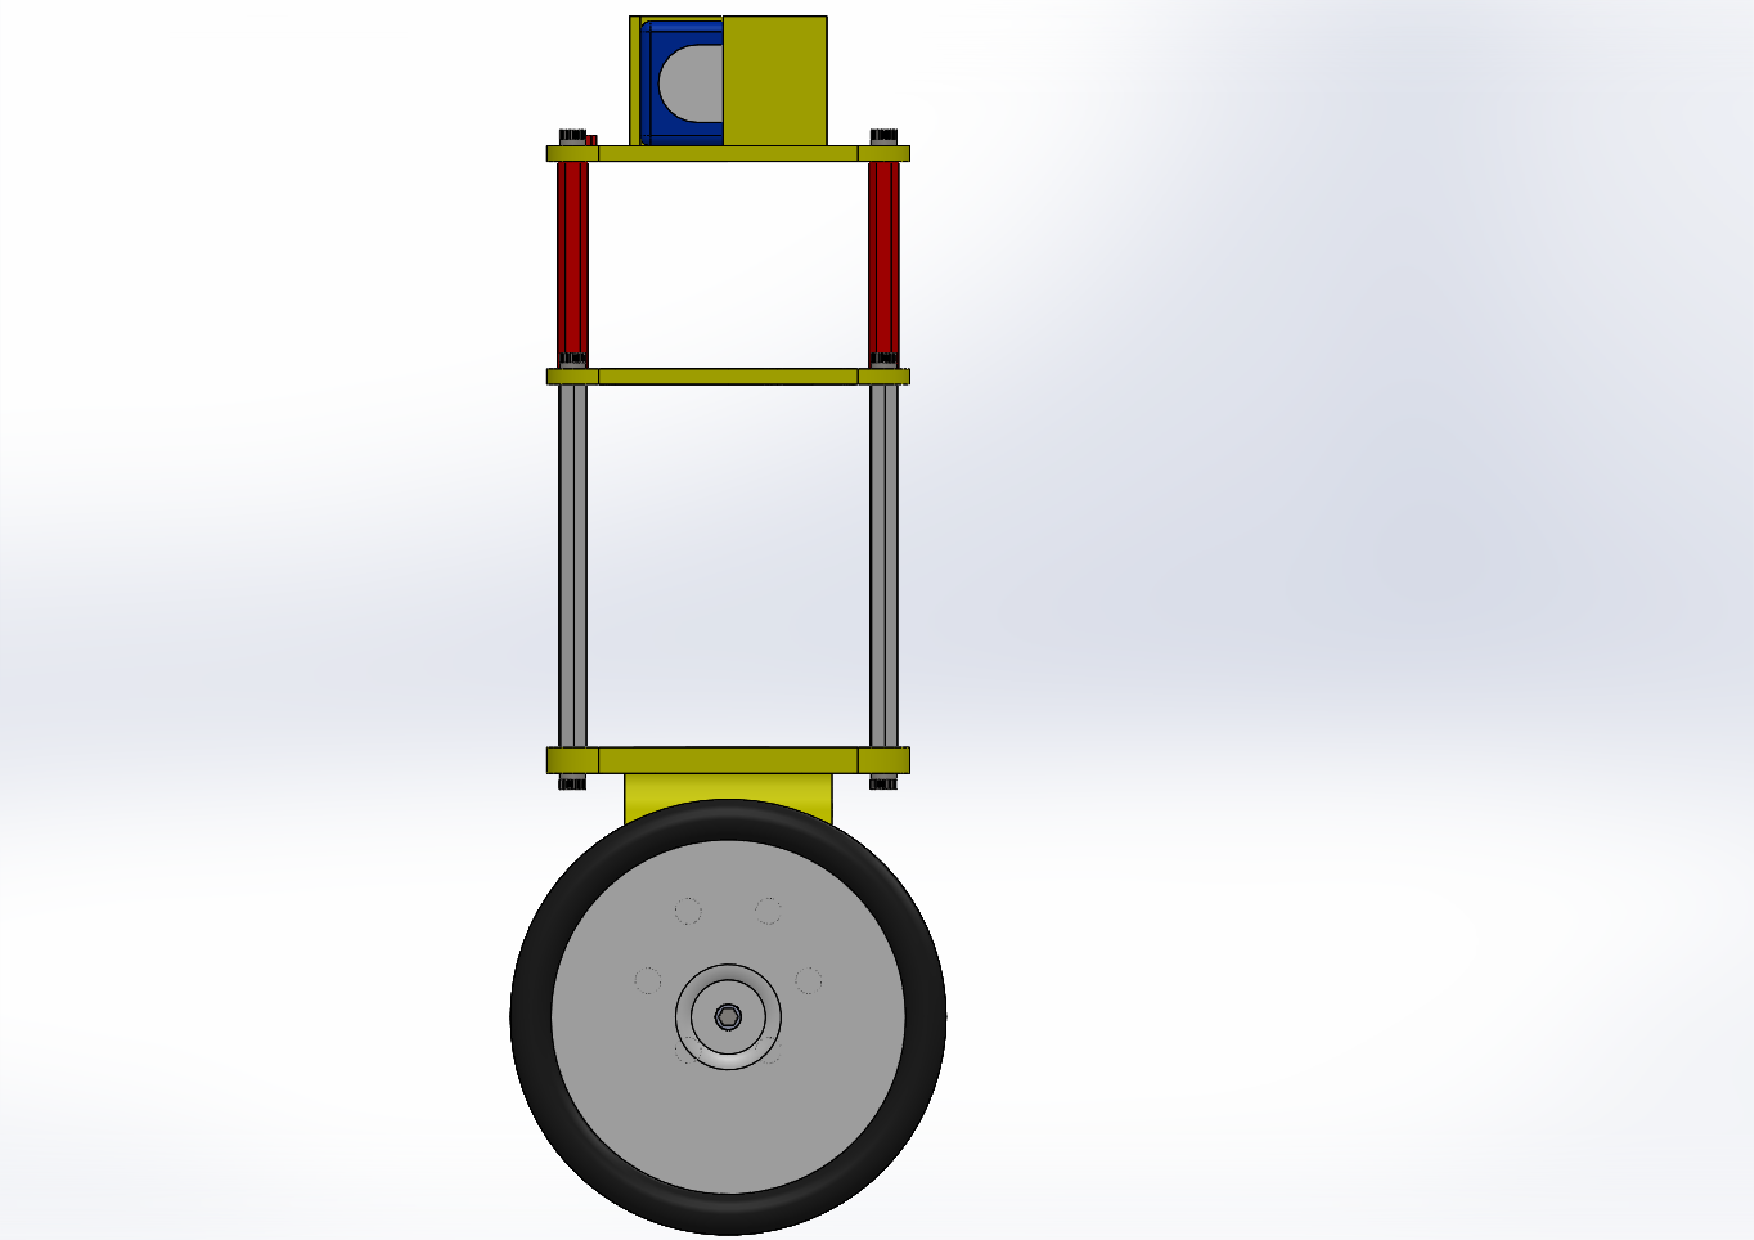
\includegraphics[trim = 5cm 0mm 10cm 0mm,clip, angle=0, scale = 0.35]{imagenes/Balancing_Robot/EnsanBalanceLateral.PDF}
	\end{figure}
\end{center}
\end{frame}

\begin{frame}{Estructura mecánica}
\begin{center}
	\begin{figure}[H]
		\center
		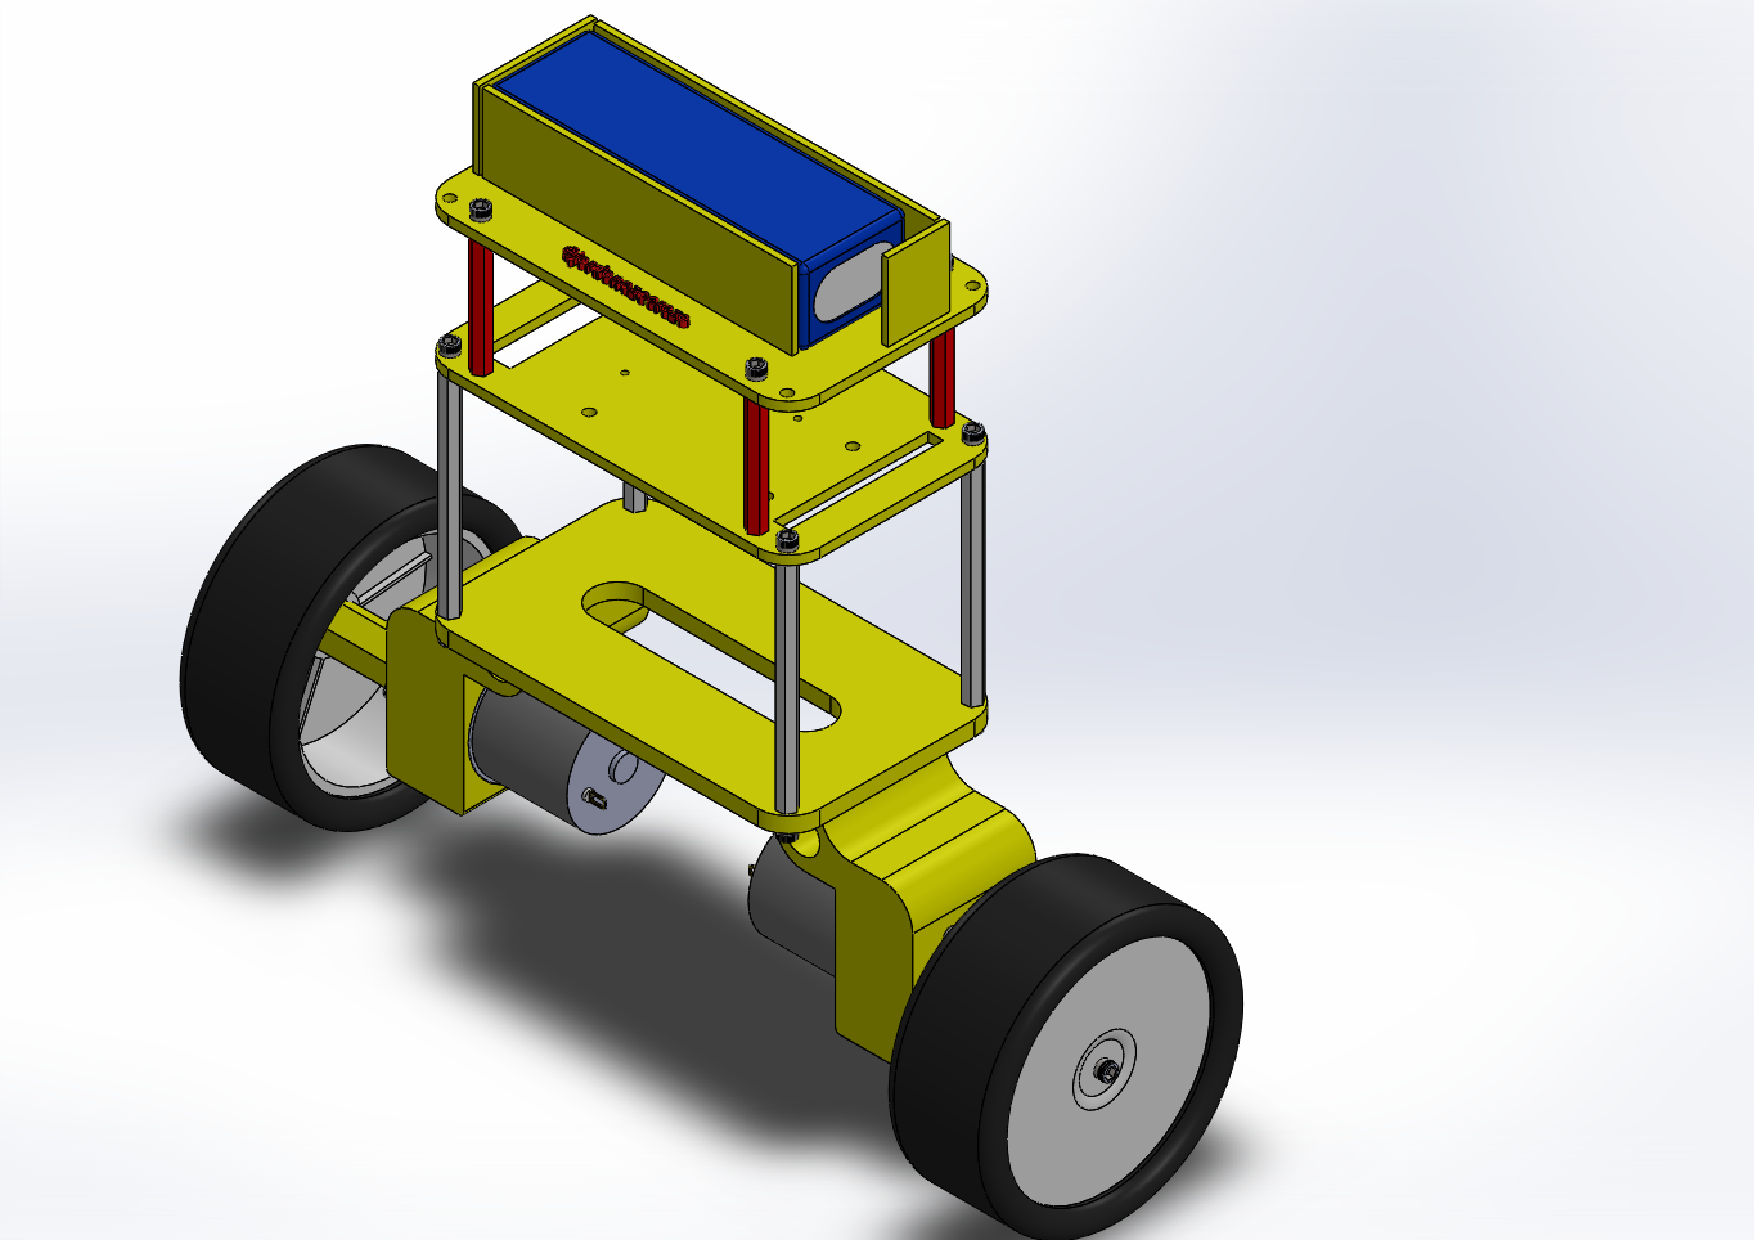
\includegraphics[trim = 2cm 0mm 8cm 0mm,clip, angle=0, scale = 0.35]{imagenes/Balancing_Robot/EnsanBalanceCab.PDF}
	\end{figure}
\end{center}
\end{frame}

\begin{frame}{Estructura mecánica}
	\begin{block}{}	
		\begin{itemize}
			\item ¿Cuál es la mejor opción para facilitar la estabilización? \pause
			\item Caracterización matemática del modelo físico \pause
			\item Centro de masas en el centro del eje vertical \pause
		\end{itemize}
	\end{block}
	\begin{alertblock}{}
		SE HACE USO DE SOLIDWORKS PARA EL DISEÑO DE LAS PIEZAS Y EL CÁLCULO DEL CENTRO DE MASAS
		\begin{center}
			
\includegraphics [width =0.4\textwidth ]{imagenes/SolidWorks-01}
		\end{center}
	\end{alertblock}


\end{frame}

\begin{frame}{Estructura mecánica}
	\begin{figure}[H]
		\center
		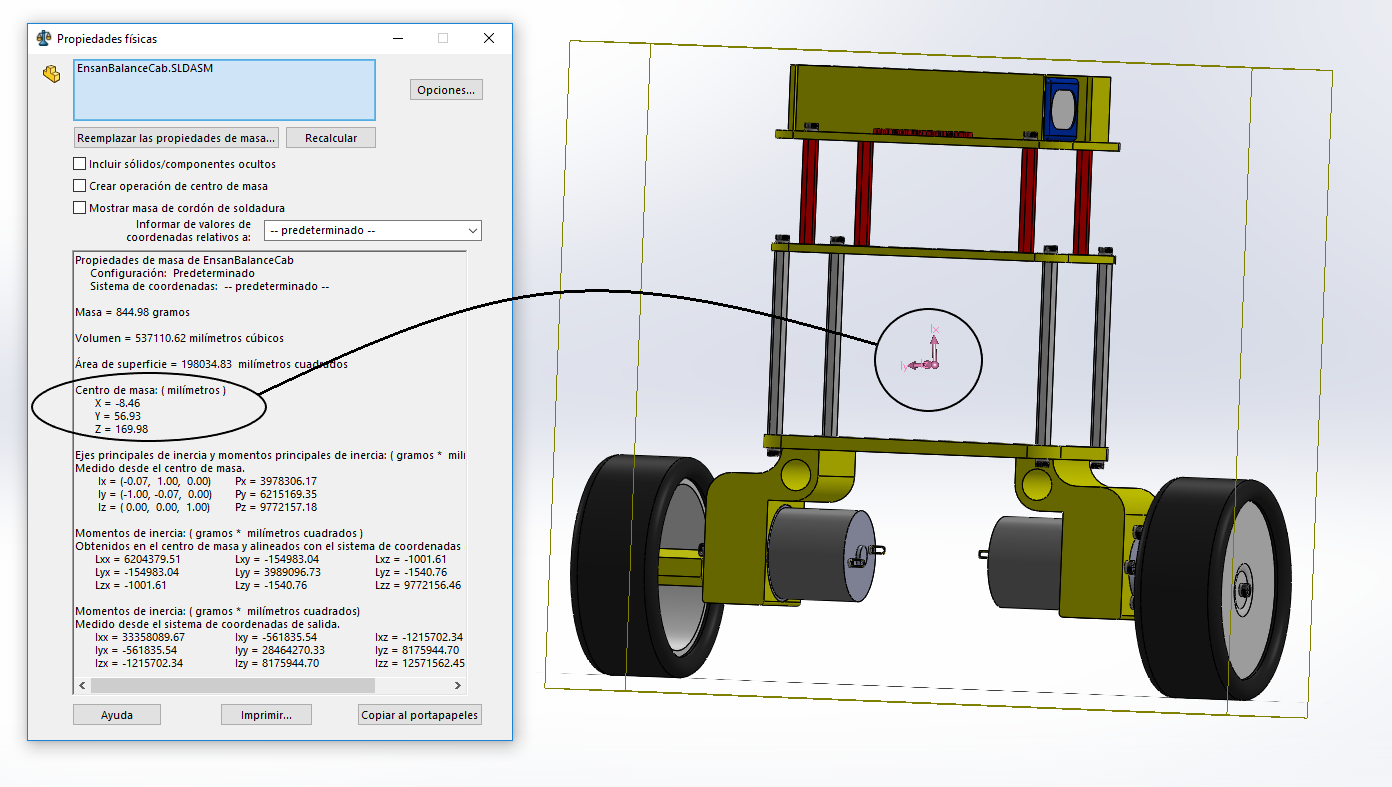
\includegraphics[scale=0.3]{imagenes/Balancing_robot/center_mass}
	\end{figure}
\end{frame}

\begin{frame}{Obtención ángulo}
\begin{block}{}
	\begin{itemize}
		\item Para corregir el ángulo es necesario el conocimiento de este en cada instante.\pause
		\item Unidad de medida incercial (IMU) \pause
	\end{itemize}
\end{block}
\begin{alertblock}{}
	\centering \textbf{MPU6050} \pause
\end{alertblock}
	\begin{center}
	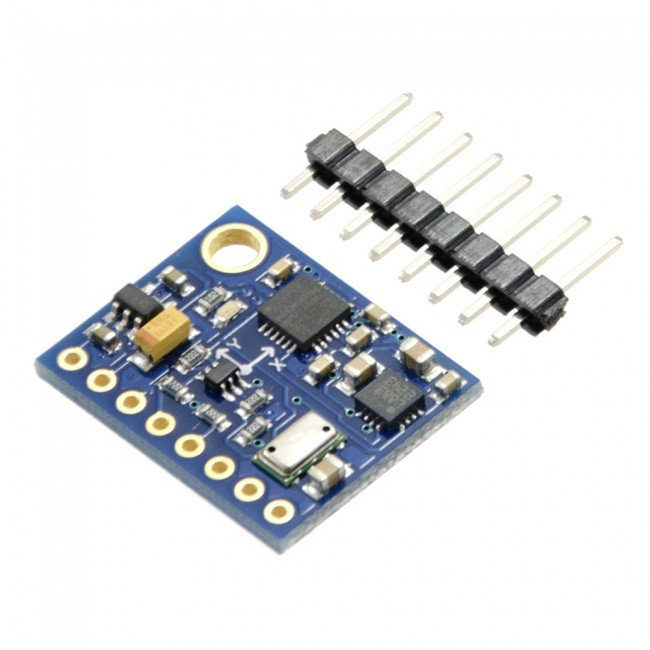
\includegraphics [width =0.3\textwidth ]{imagenes/EstadoArte/IMU1}
\end{center}
\end{frame}

\begin{frame}{Obtención ángulo}
		\begin{block}{}
			\begin{itemize}
				\item 6DOF \pause
				\item Acelerómetro y giroscopio \pause
				\item Comunicación I2C \pause
				\item Uso de DMP solo para Arduino \pause
			\end{itemize}
		\end{block}
		\begin{alertblock}{}
			\centering \textbf{MEJOR OPCIÓN CON ARDUINO} 
		\end{alertblock}
\end{frame}

\begin{frame}{Obtención ángulo}
	\begin{figure}[H]
		\center
		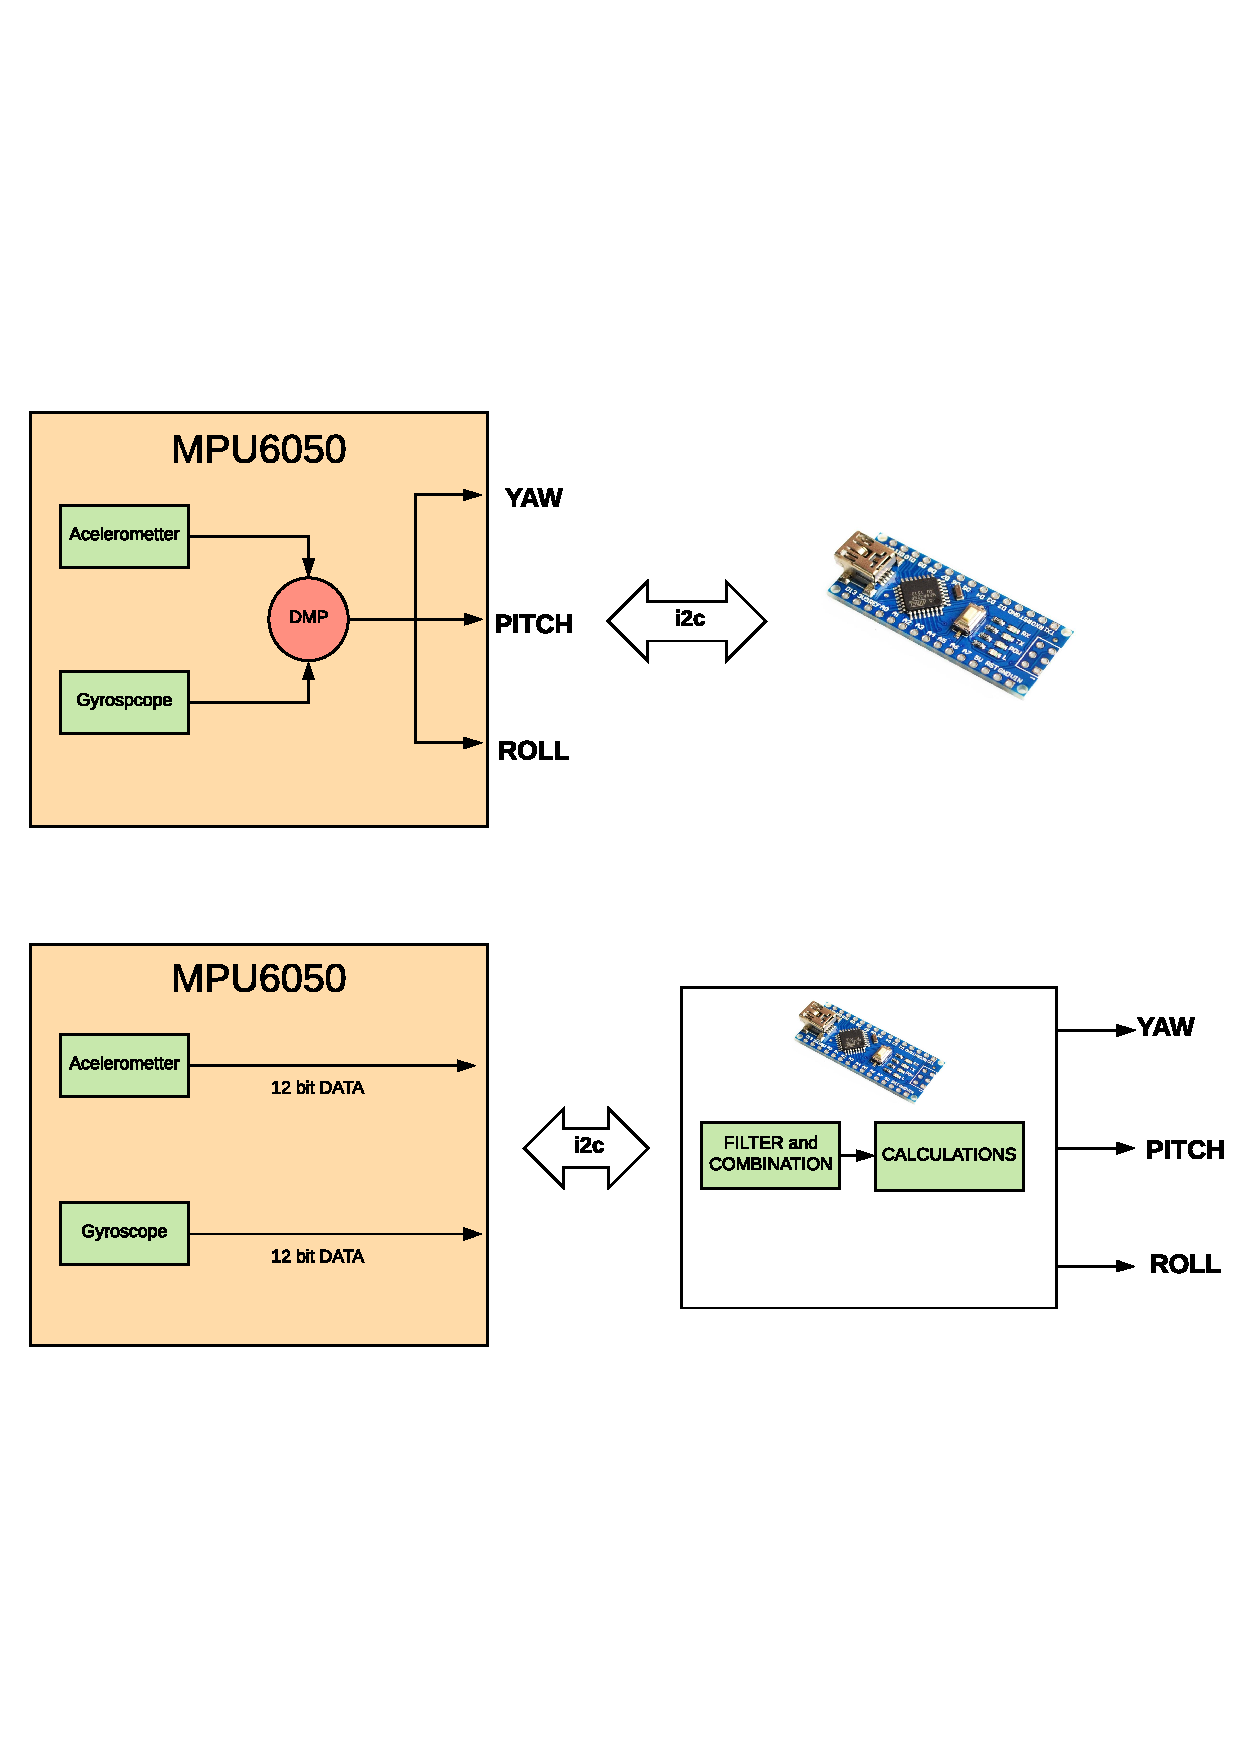
\includegraphics[trim = 0mm 5cm 0mm 5cm, clip,scale=0.4]{imagenes/Balancing_robot/DMPexample.pdf}
	\end{figure} 
\end{frame}


\begin{frame}{Coexistencia microcontrolador-FPGA}
\begin{block}{}
	\begin{itemize}
		\item Ángulo obtenido por Arduino-Nano \pause
		\item FPGA necesita conocer el ángulo \pause
	\end{itemize}
\end{block}
\begin{alertblock}{}
	\centering \textbf{Coexistencia microcontrador-FPGA}  \pause
\end{alertblock}
\begin{alertblock}{}
	\centering \textbf{Paralelizar los procesos que pueden ser paralelizados} \pause 
\end{alertblock}
\end{frame}


\begin{frame}{Coexistencia microcontrolador-FPGA}
	\begin{figure}[H]
		\center
		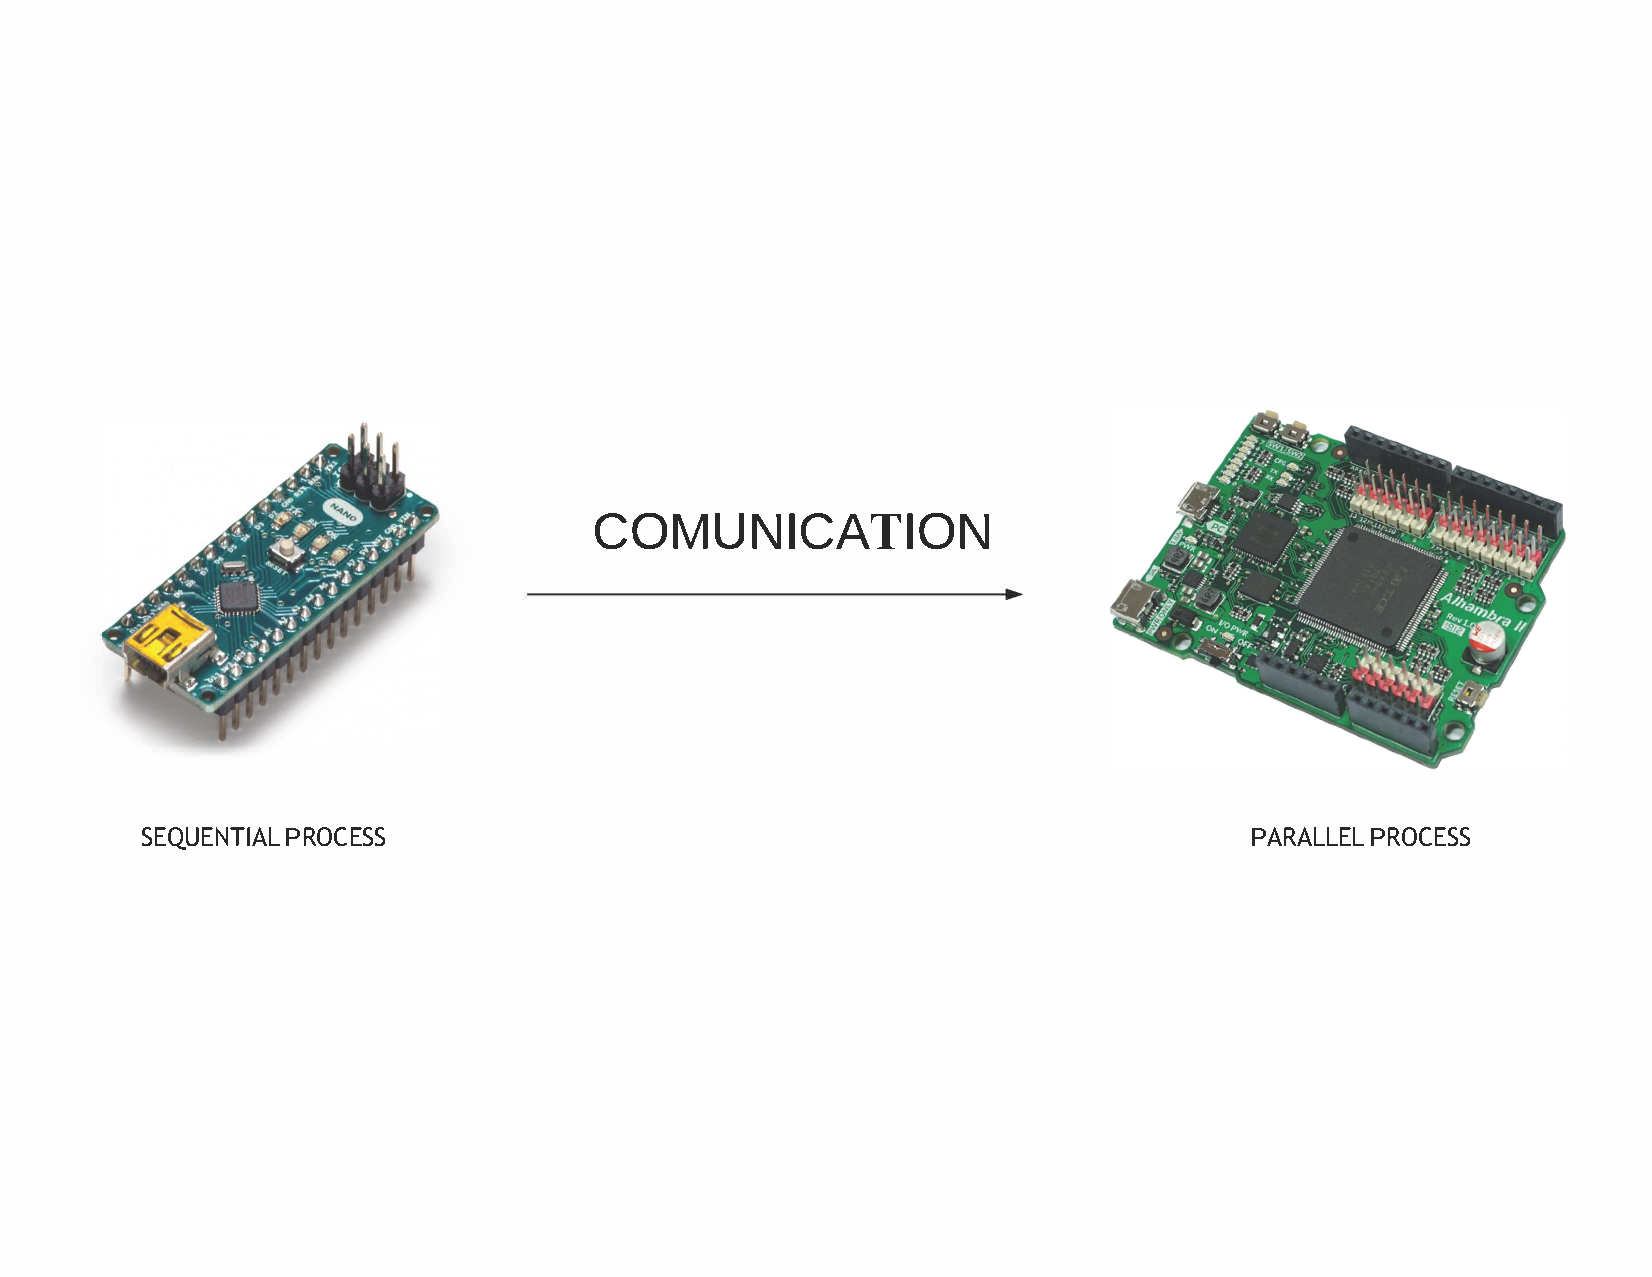
\includegraphics[trim = 0mm 40mm 0mm 20mm, clip,scale=0.4]{imagenes/Balancing_robot/coexistencia1.pdf}
	\end{figure}
\end{frame}

\begin{frame}{Coexistencia microcontrolador-FPGA}
\begin{figure}[H]
	\center
	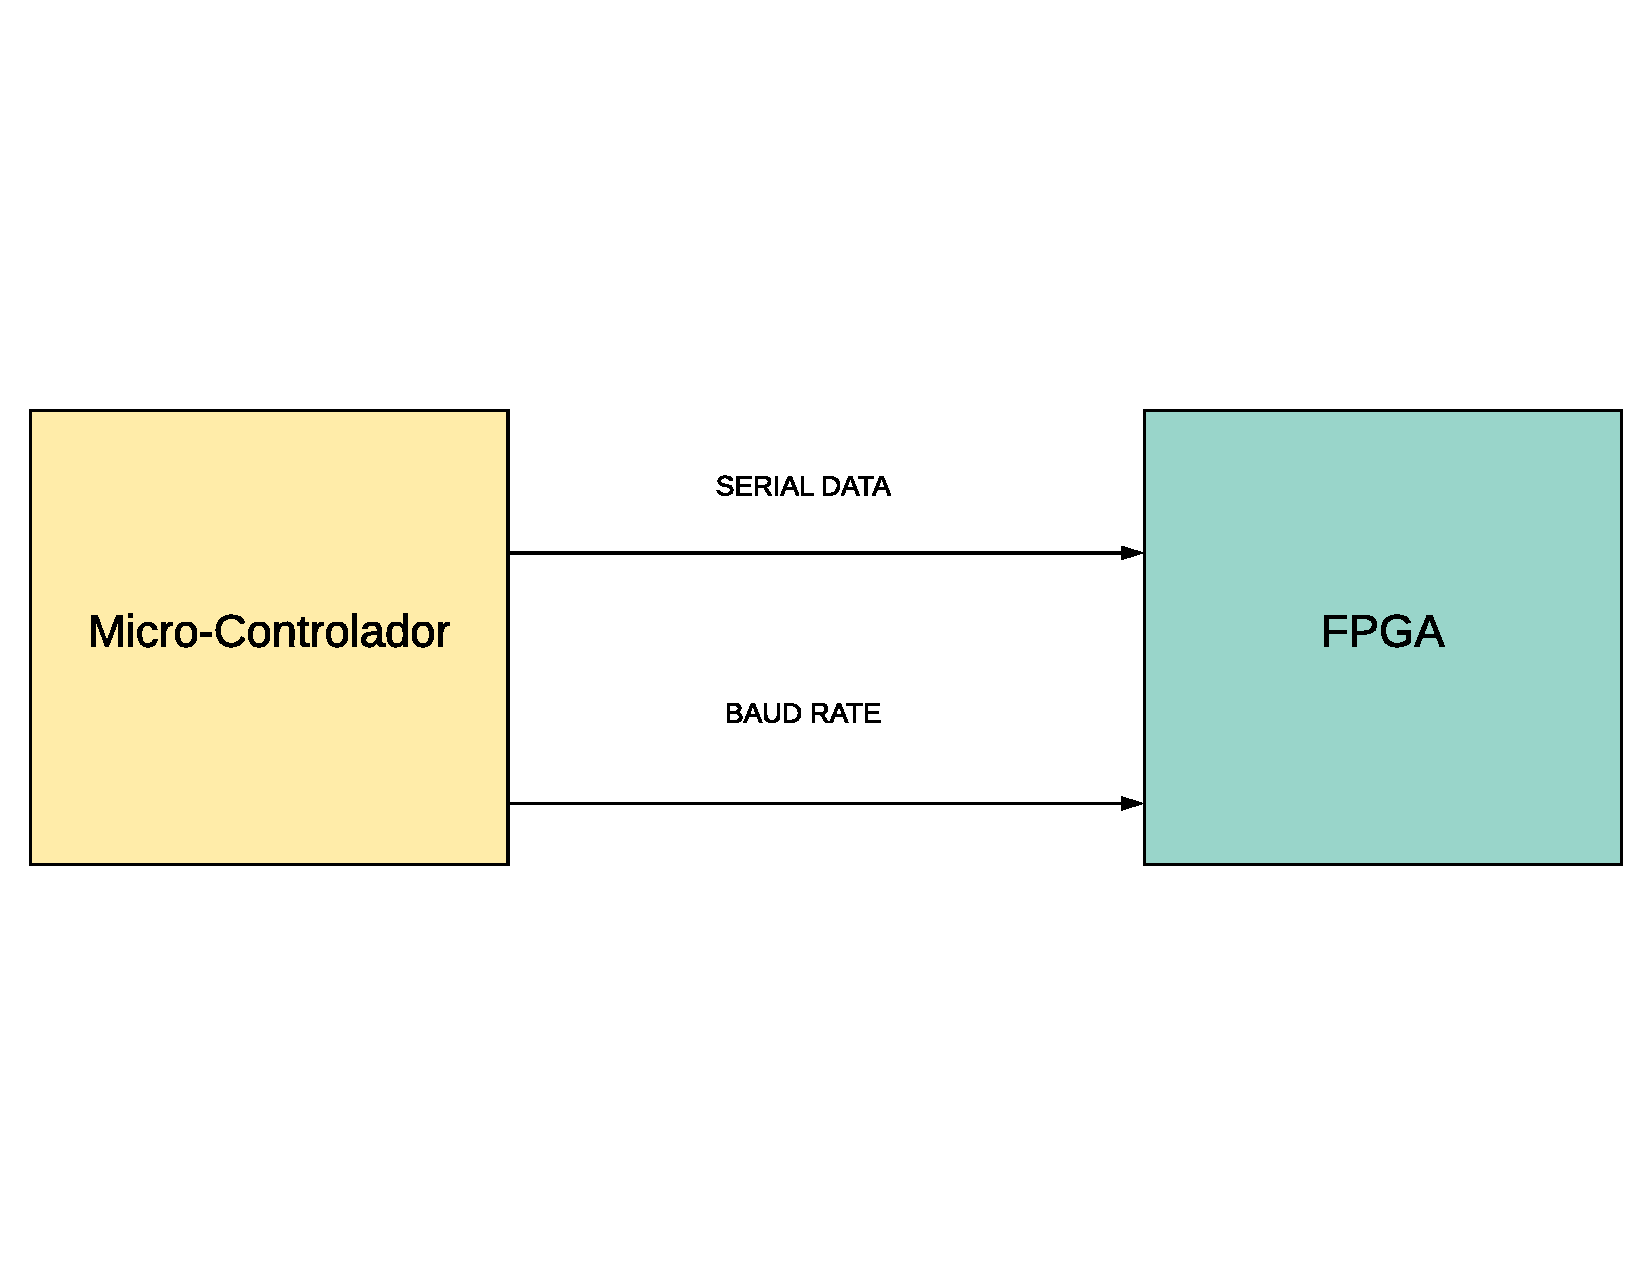
\includegraphics[trim = 0mm 40mm 0mm 20mm, clip,scale=0.3]{imagenes/Balancing_robot/coexistencia2.pdf}
\end{figure}
\begin{center}
	\begin{figure}[H]
		\center
		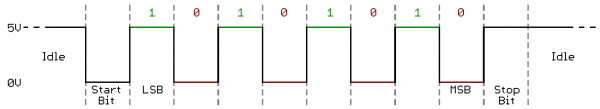
\includegraphics[scale=0.75, angle=0]{imagenes/Balancing_Robot/serial_comunicattion.png}
	\end{figure}
\end{center}
\end{frame}

\begin{frame}{Coexistencia microcontrolador-FPGA}
		\centering \textbf{Desde el punto de vista del microcontrolador}
		\begin{figure}[H]
			\center
			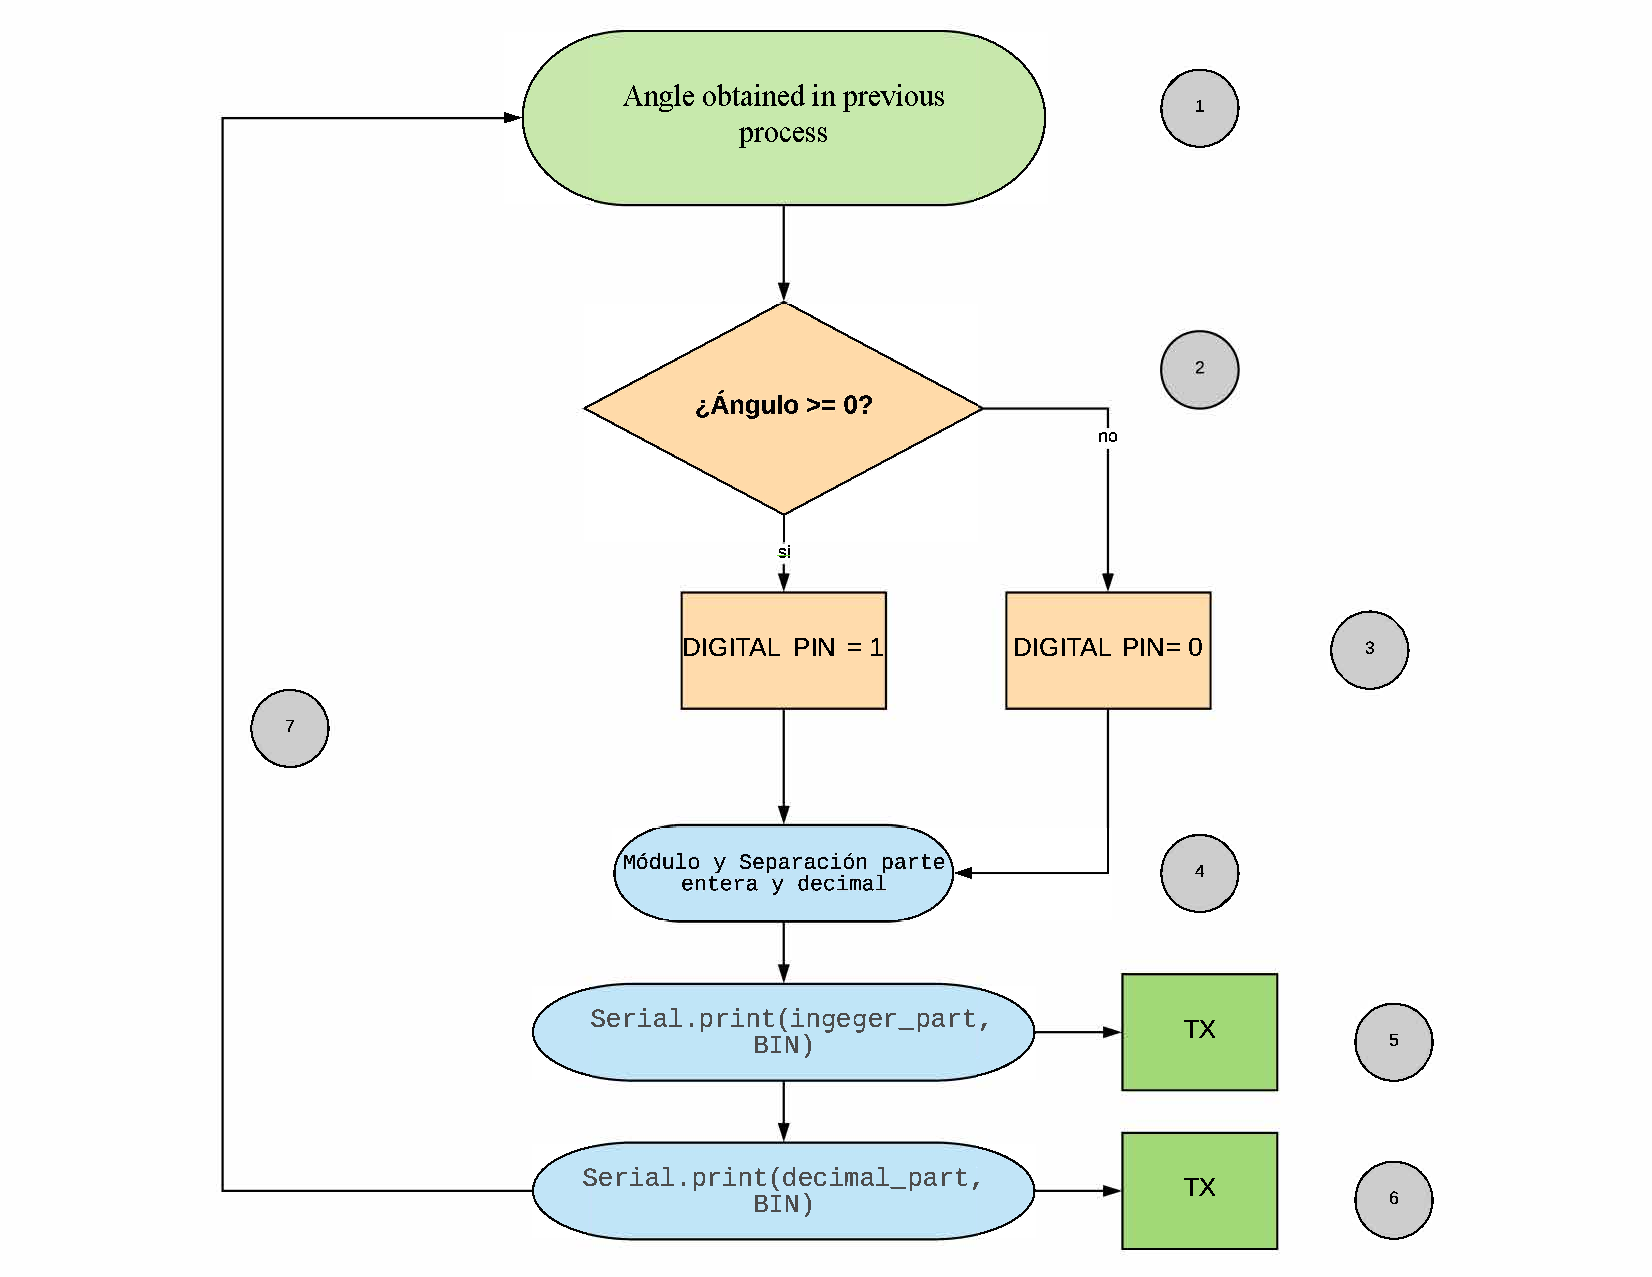
\includegraphics[trim = 0mm 0mm 0mm 0mm, clip,scale=0.3]{imagenes/Balancing_robot/extraccion_angulo.pdf}
		\end{figure}
\end{frame}

\begin{frame}{Coexistencia microcontrolador-FPGA}
\centering \textbf{Desde el punto de vista de la FPGA}
\begin{center}
	\begin{figure}[H]
		\center
		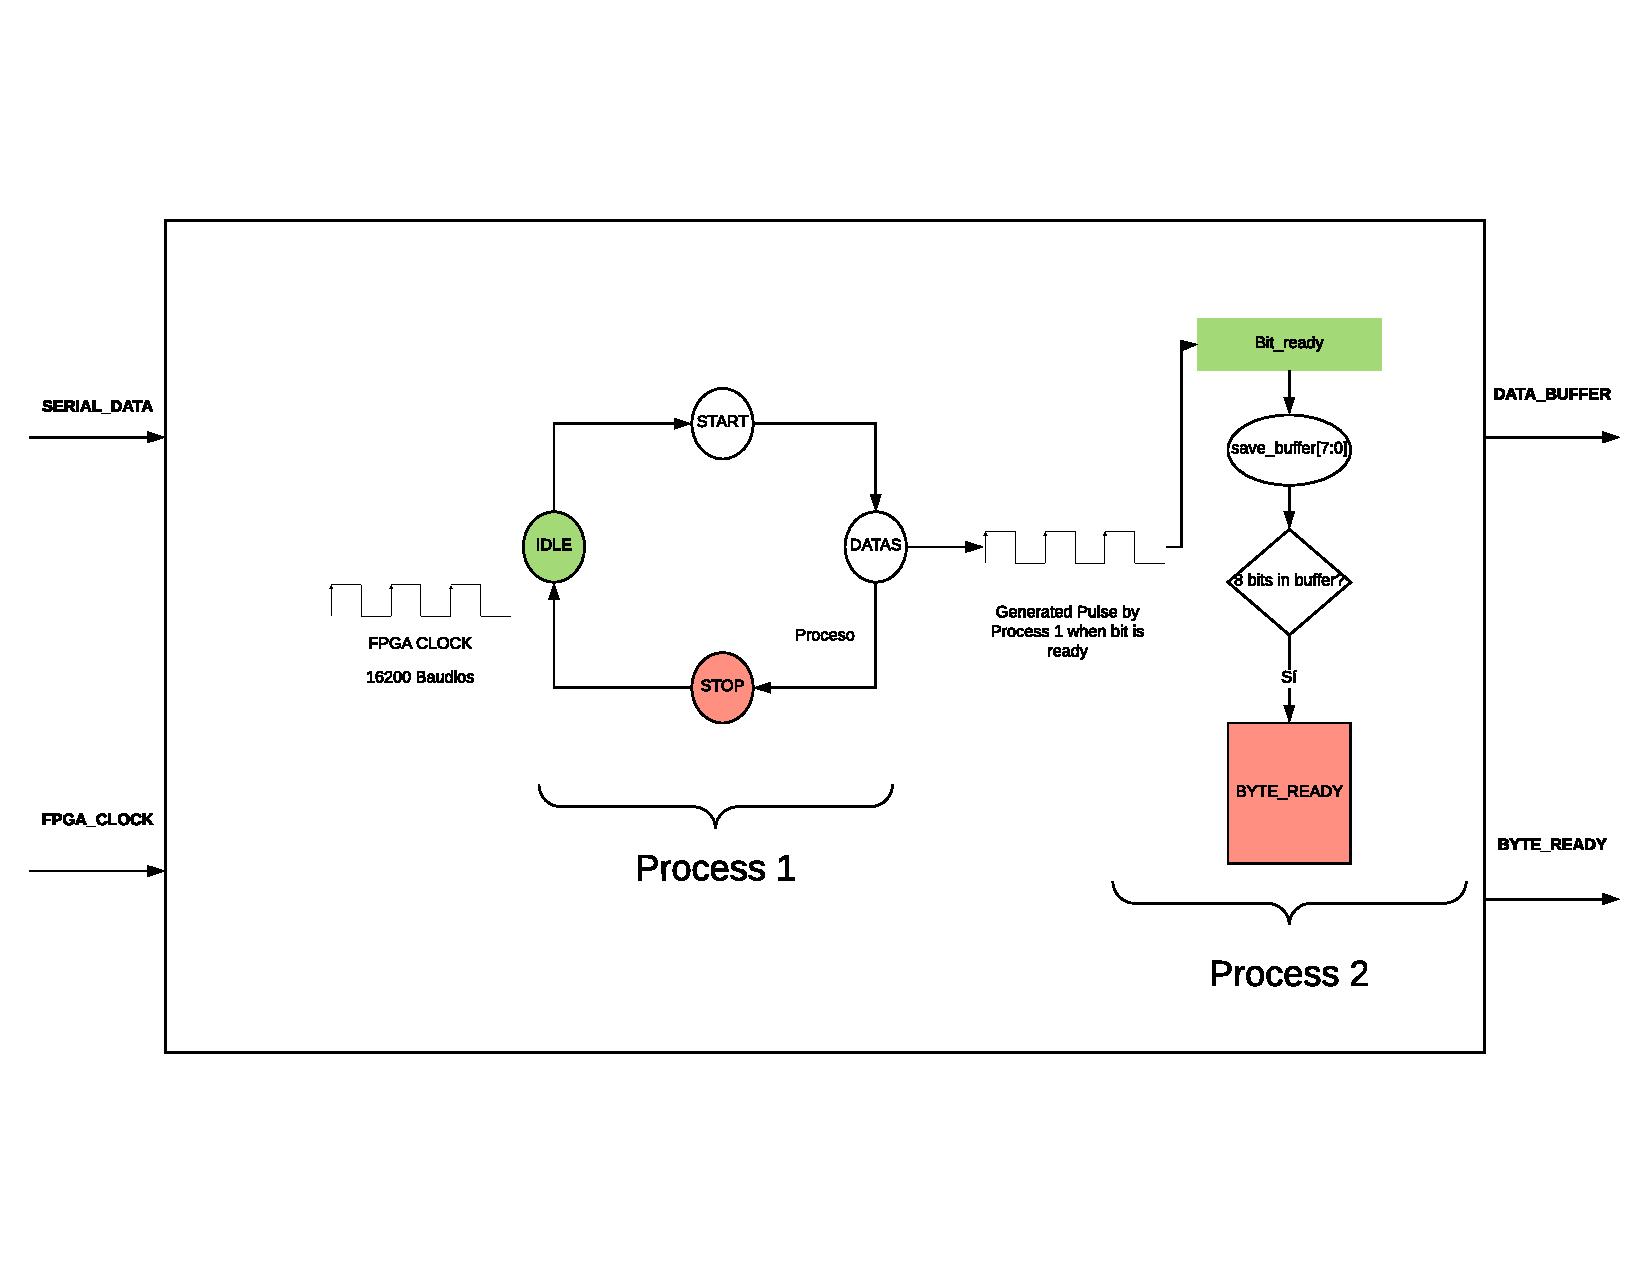
\includegraphics[trim = 0mm 0mm 0mm 10mm, clip,scale=0.4, angle=0]{imagenes/Balancing_robot/arduino_interfacefluid.pdf}

	\end{figure}
\end{center}
\end{frame}

\begin{frame}{Coexistencia microcontrolador-FPGA}
\centering \textbf{Aspecto en IceStudio de la comunicación}
\begin{figure}[H]
	\center
	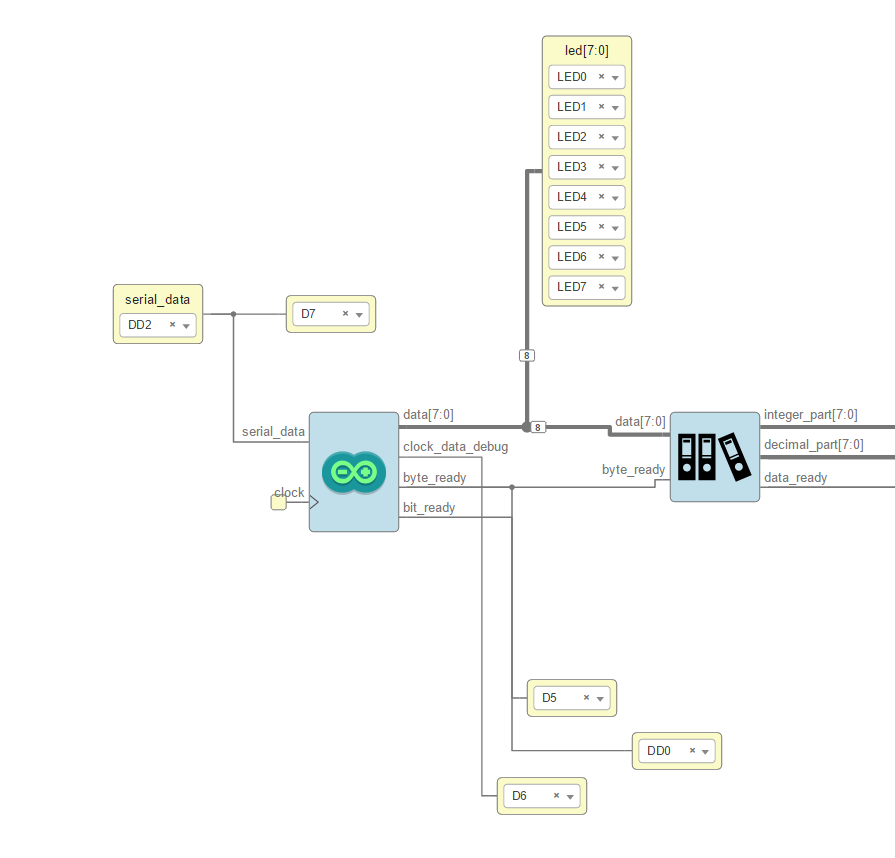
\includegraphics[scale=0.3]{imagenes/Balancing_robot/arduino_arrange.PNG}
\end{figure}
\end{frame}





\begin{frame}{Control PID}
\begin{block}{}
	\begin{itemize}
		\item Necesidad de minimizar el ángulo, en este caso a 0º
		\item Surgen muchas opciones, lógica fuzzy, algoritmos genéticos, PID
		\item PID por su fácil implementación y paralelismo
	\end{itemize}
\end{block}
\begin{alertblock}
	\centering \textbf{PID por su fácil implementación y paralelismo}
\end{alertblock}
\end{frame}

\begin{frame}{Control P}
		\begin{figure}[H]
		\center
		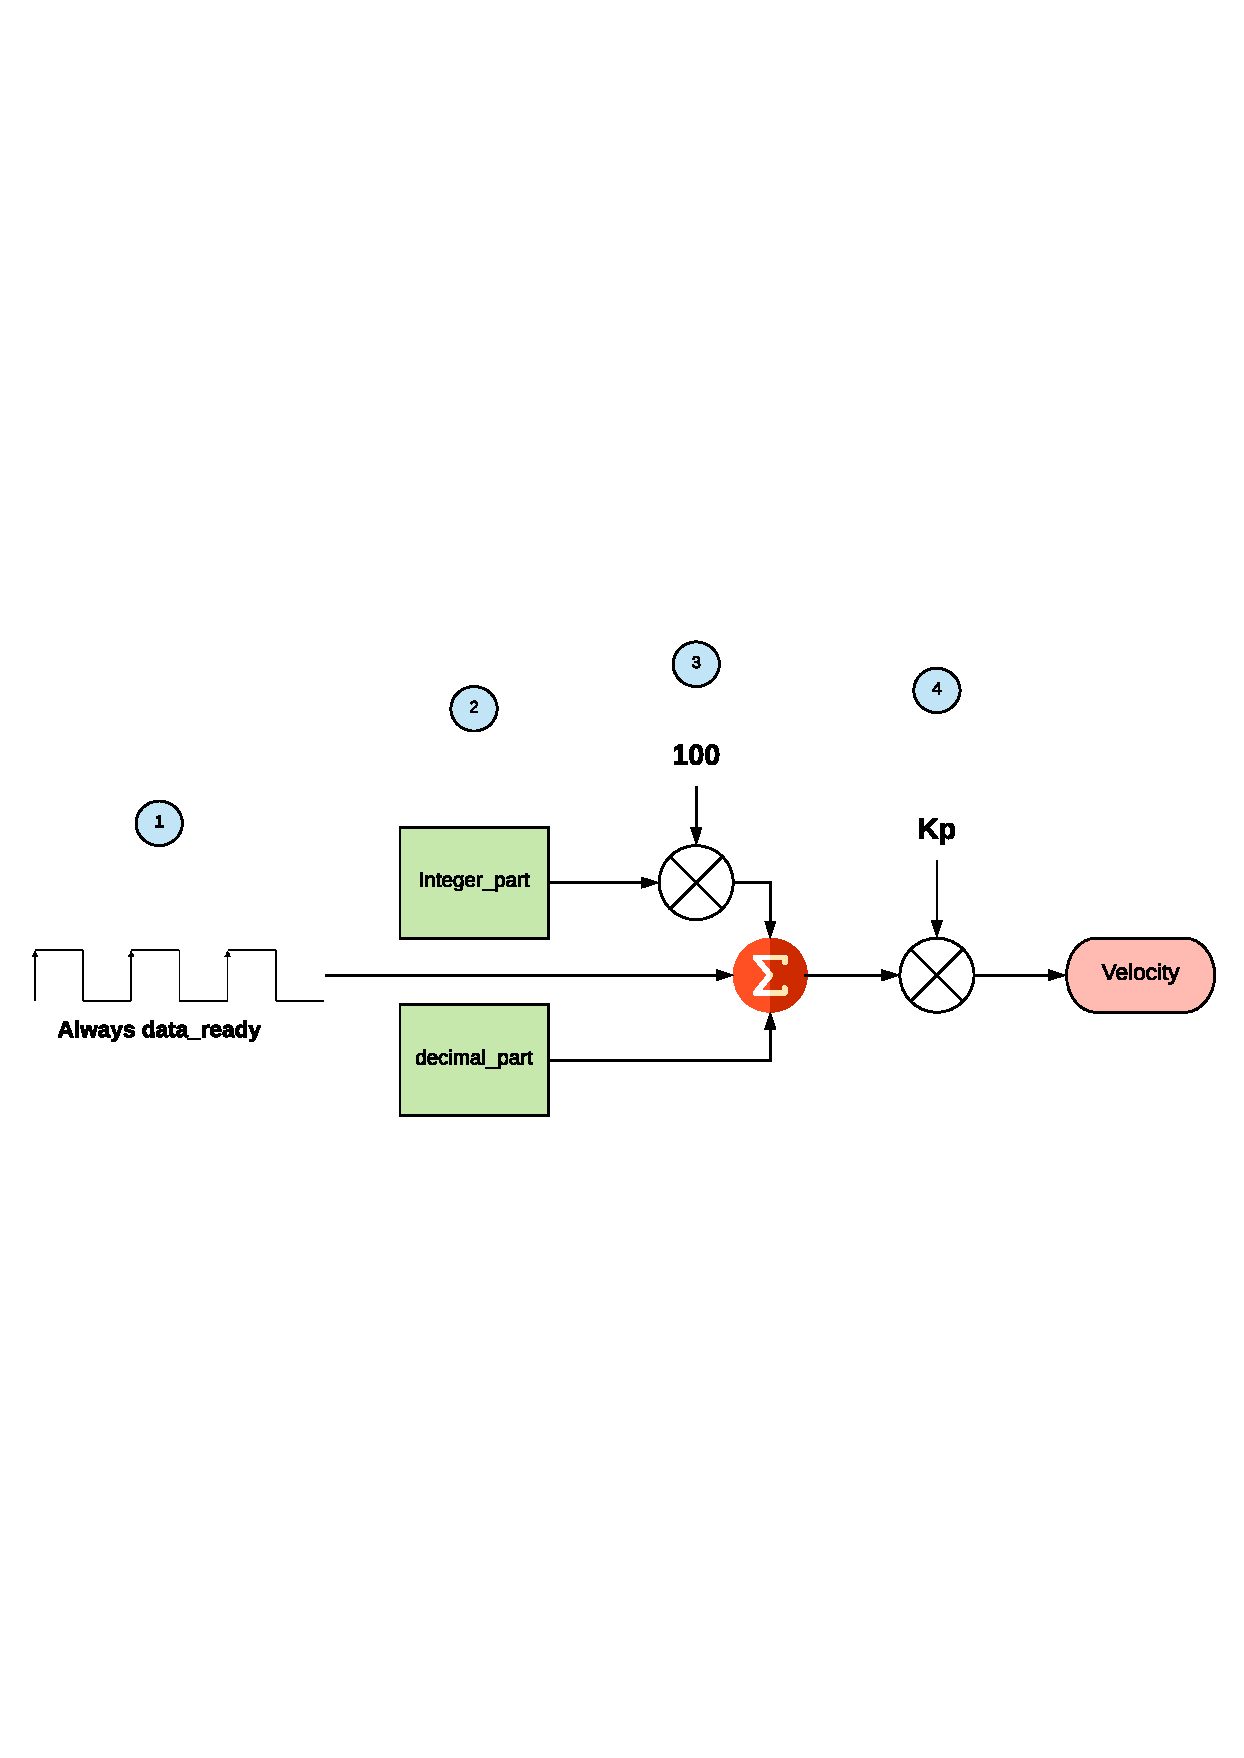
\includegraphics[trim = 0cm 7cm 0mm 7cm, clip,scale=0.5]{imagenes/Balancing_robot/P.pdf}
		\end{figure}
\end{frame}

\begin{frame}{Control D}
			\begin{figure}[H]
			\center
			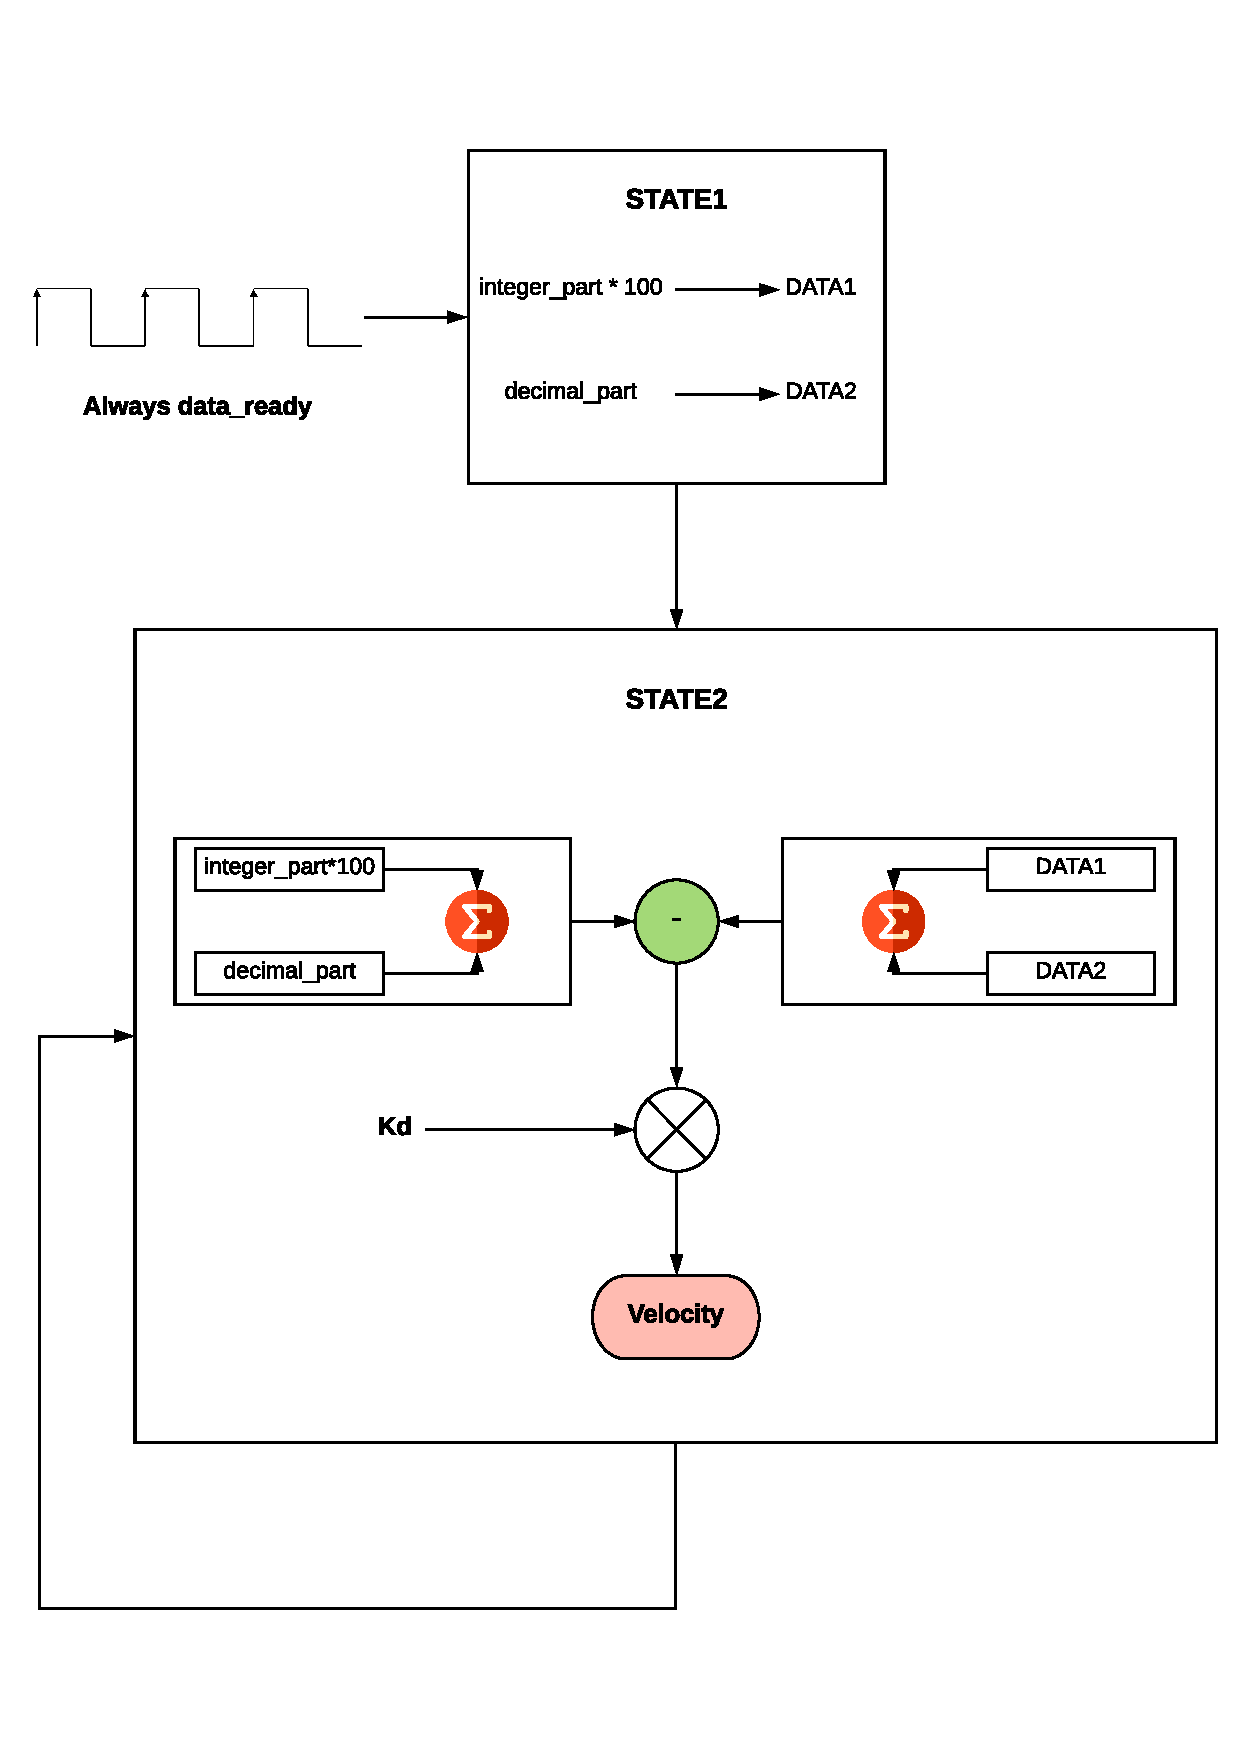
\includegraphics[trim = 0cm 0cm 0mm 2cm, clip,scale=0.3]{imagenes/Balancing_robot/D.pdf}
		\end{figure}
\end{frame}

\begin{frame}{Control PD}
	\begin{figure}[H]
		\center
		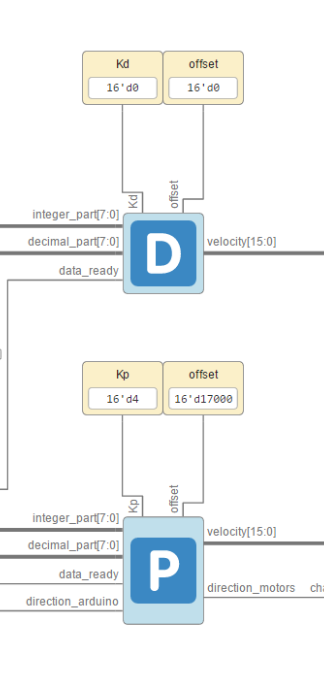
\includegraphics[trim = 0cm 0cm 0mm 0cm, clip,scale=0.5]{imagenes/Balancing_robot/PDControl.PNG}
	\end{figure}
\end{frame}



\begin{frame}{Control de los motores}
\begin{block}{}
	\begin{itemize}
		\item Traducción de la salida del PD, velocidad y sentido de motores DC \pause
	\end{itemize}
\end{block}
\centering \textbf{MC33926}
		\begin{figure}[H]
			\center
			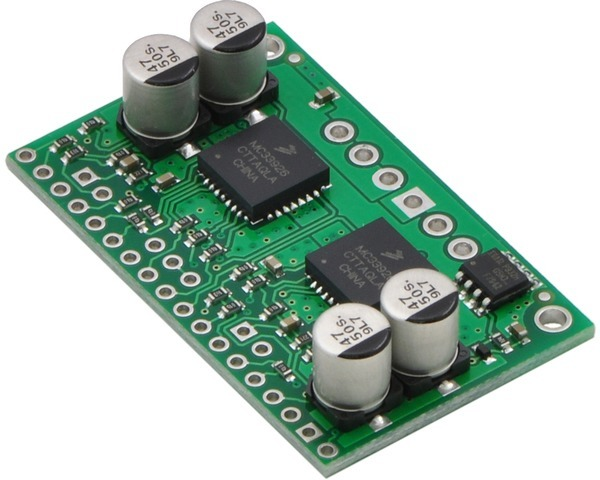
\includegraphics[trim = 0mm 0cm 0mm 0cm, clip,scale=0.2]{imagenes/Balancing_robot/driver_motor.jpg} \pause
		\end{figure}

\begin{alertblock}{}
	\begin{itemize}
		\item Como entradas: \begin{itemize}
			\item Señal PWM \pause
			\item Sentido de giro \pause
		\end{itemize}
		\item Como salidas: \begin{itemize}
		\item Movimiento de los motores 
	\end{itemize}
	\end{itemize}
\end{alertblock}
\end{frame}


\begin{frame}{Módulo PWM}
	\begin{figure}[H]
		\center
		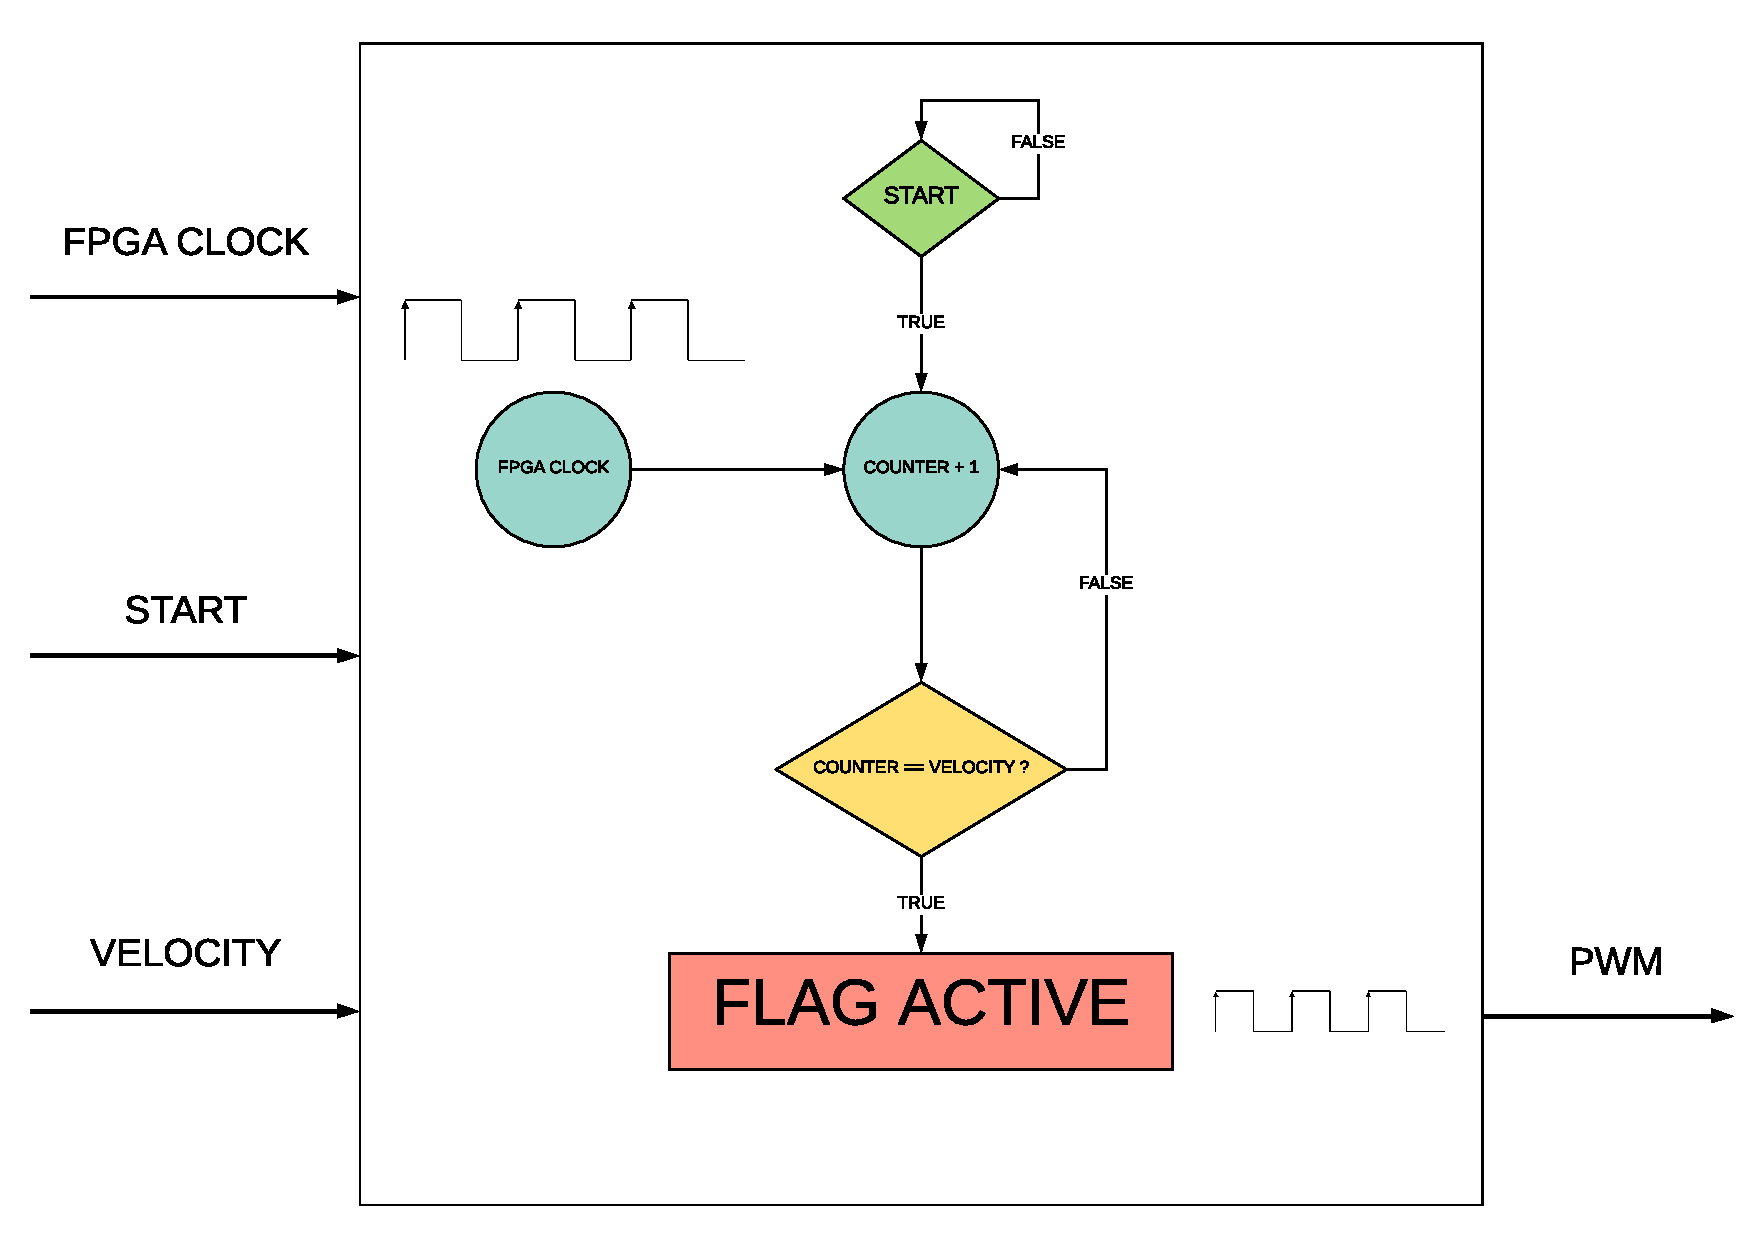
\includegraphics[trim = 0mm 0mm 0mm 0mm, clip,scale=0.35]{imagenes/Balancing_robot/pwm_control.pdf}
	\end{figure}
\end{frame}

\begin{frame}{Módulo PWM}
	\begin{figure}[H]
		\center
		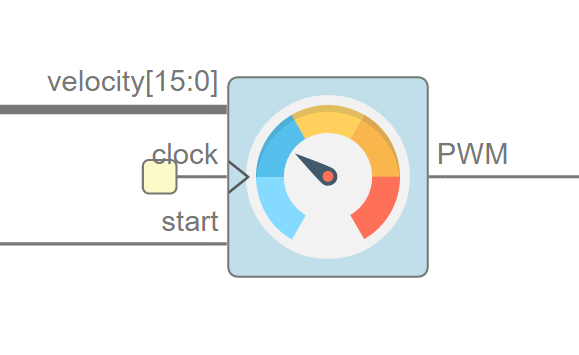
\includegraphics[scale=0.5]{imagenes/Balancing_robot/PWM_module.PNG}
	\end{figure}
\end{frame}


\begin{frame}{Diseño e Implementación PCB}
\begin{block}{}
	\begin{itemize}
		\item Demasiados cables sueltos y puentes en el sistema final \pause
		\item Necesidad de englobarlo todo en un sistema único y compacto \pause
		\item Que resuelva problemas de ruido y referencia de tierra. \pause
	\end{itemize}
\end{block}
\begin{alertblock}{}
	\centering \textbf{Printed Circuit Board, PCB} \pause
	\begin{center}
		
\includegraphics [width =0.4\textwidth ]{imagenes/altium}
	\end{center}
\end{alertblock}
\end{frame}

\begin{frame}{Diseño e Implementación PCB}
\begin{figure}[H]
	\center
	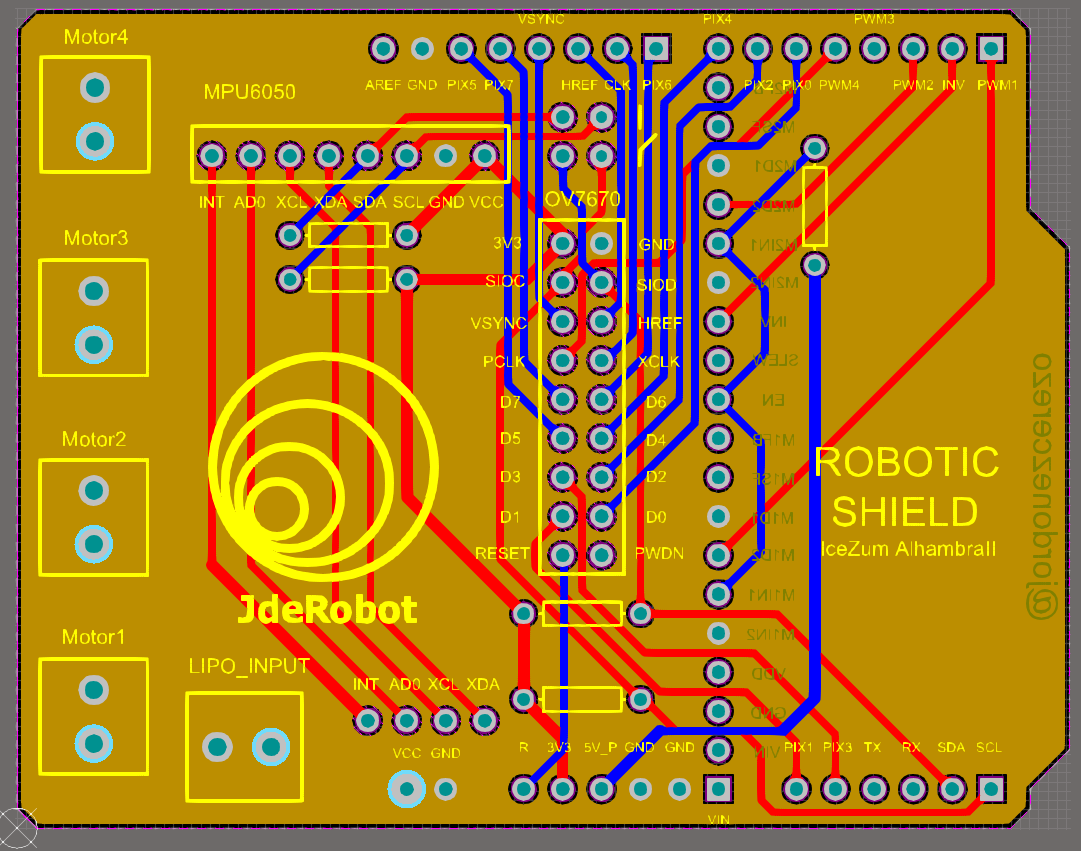
\includegraphics[scale=0.35, angle=0]{imagenes/Balancing_Robot/layers_altium.PNG}
\end{figure}
\end{frame}


\begin{frame}{Diseño e Implementación PCB}
	\begin{figure}[H]
		\center
		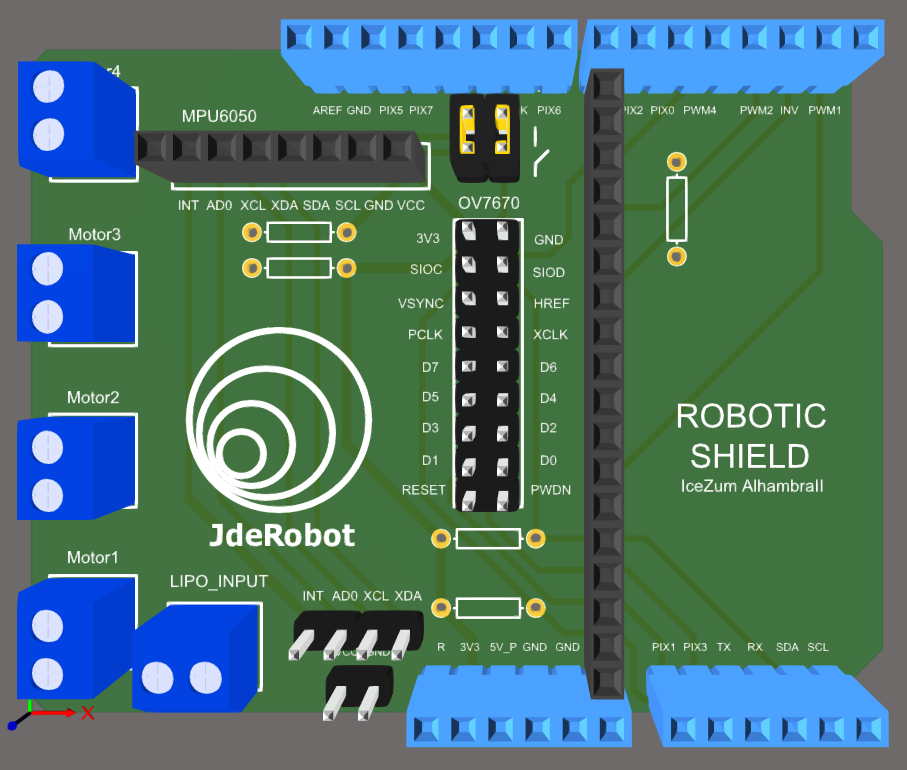
\includegraphics[scale=0.45]{imagenes/Balancing_Robot/top_3D.PNG}
	\end{figure}
\end{frame}

\begin{frame}{Diseño e Implementación PCB}
		\begin{figure}[H]
	\center
	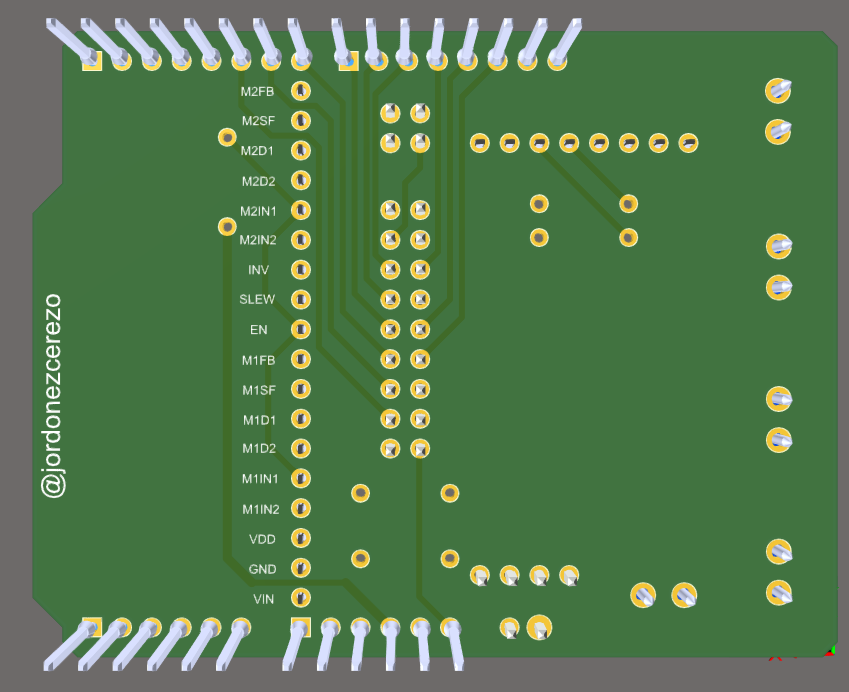
\includegraphics[scale=0.45]{imagenes/Balancing_Robot/bottom_3D.PNG}
\end{figure}
\end{frame}

\begin{frame}{Diseño e Implementación PCB}
		\begin{figure}[H]
	\center
	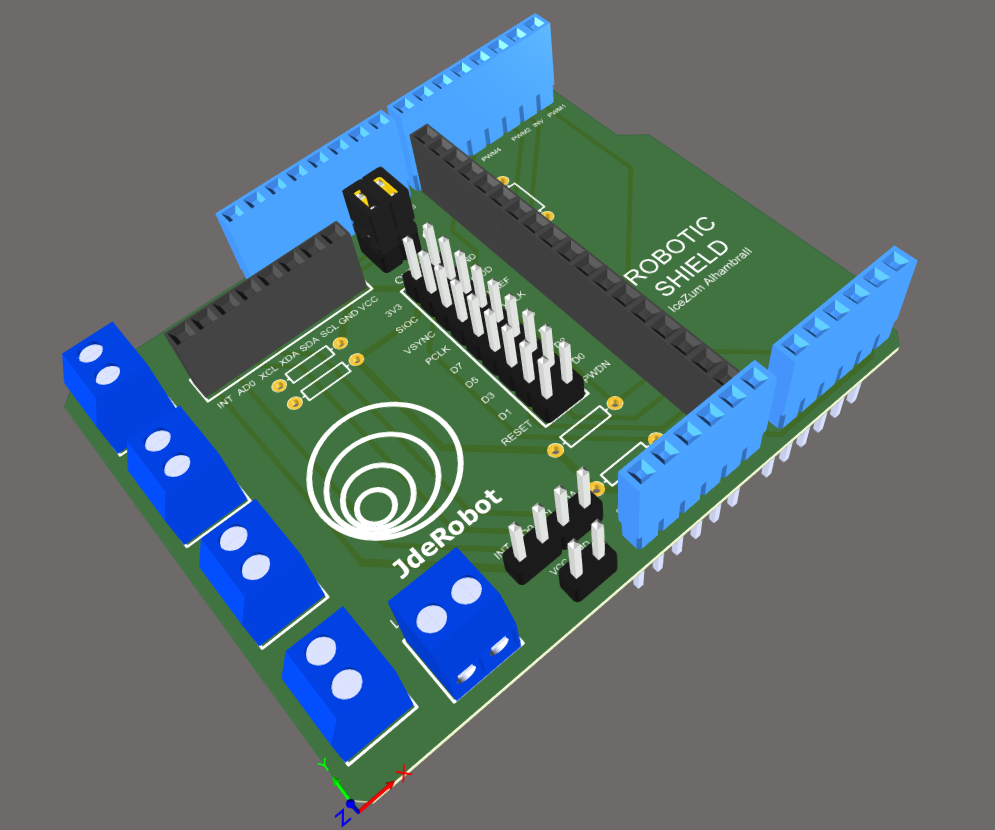
\includegraphics[scale=0.40]{imagenes/Balancing_Robot/Vista3D1.PNG}
\end{figure}
\end{frame}

\begin{frame}{Diseño e Implementación PCB}
	\begin{center}
	\begin{figure}[H]
		\center
		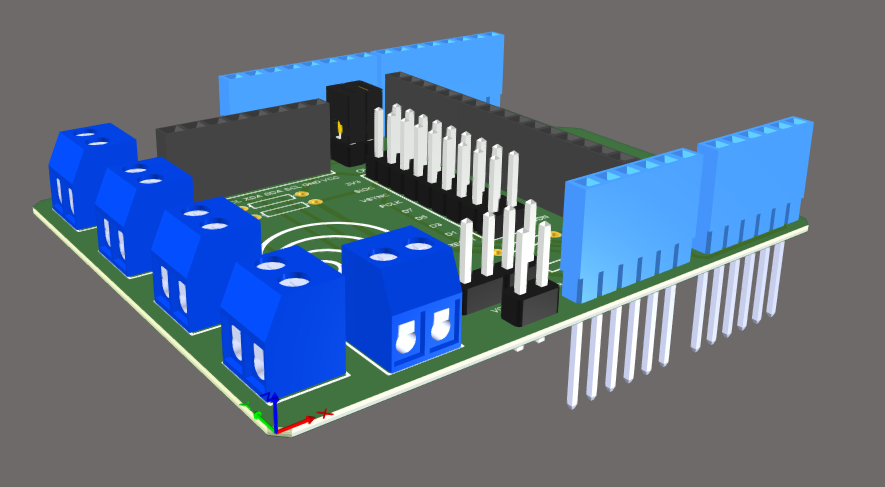
\includegraphics[scale=0.5]{imagenes/Balancing_Robot/Vista3D2.PNG}
	\end{figure}
\end{center}
\end{frame}

\subsection{Ensamblado y sistema final}
\begin{frame}{Ensamblado y sistema final}
	\begin{figure}[H]
		\center
		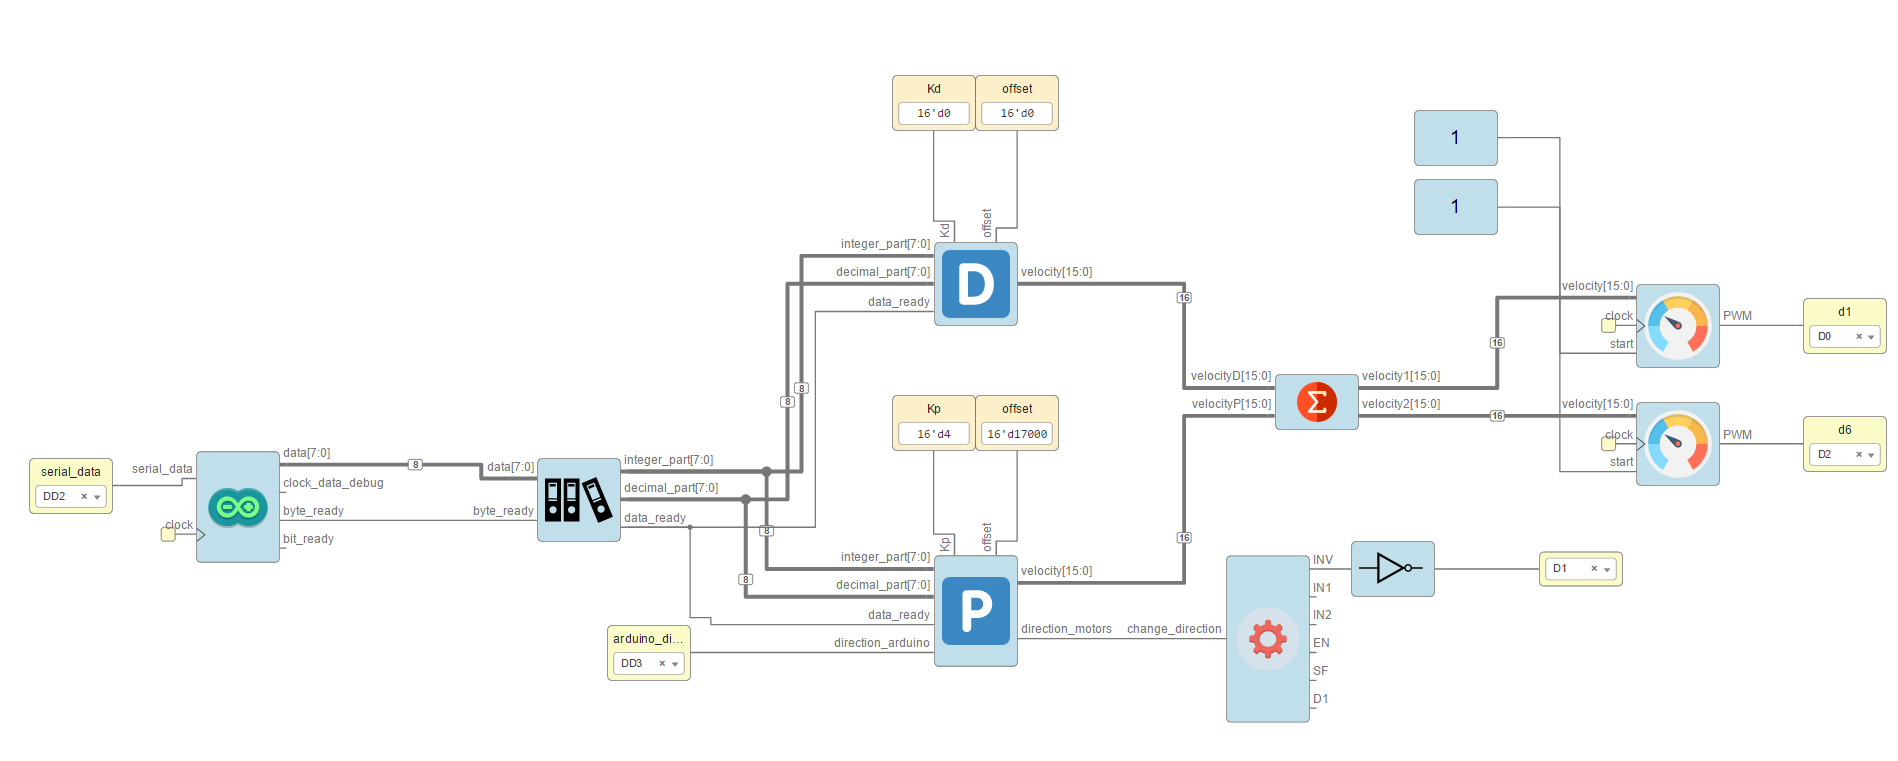
\includegraphics[scale=0.3, angle=0]{imagenes/Balancing_robot/finalIceStudio}
	\end{figure}
\end{frame}

\begin{frame}{Ensamblado y sistema final}

\end{frame}
%%%%%%%%%%%%%%%%%%%%%%%%%%%%%%%%%%%%%%%%%%%%%%%%%%%%%%%%%%%%%%%%%%%%
\section{Cuadricóptero con visión artificial}

\subsection{Diseño del sistema}

\begin{frame}{Diseño del sistema}
\begin{figure}[H]
	\center
	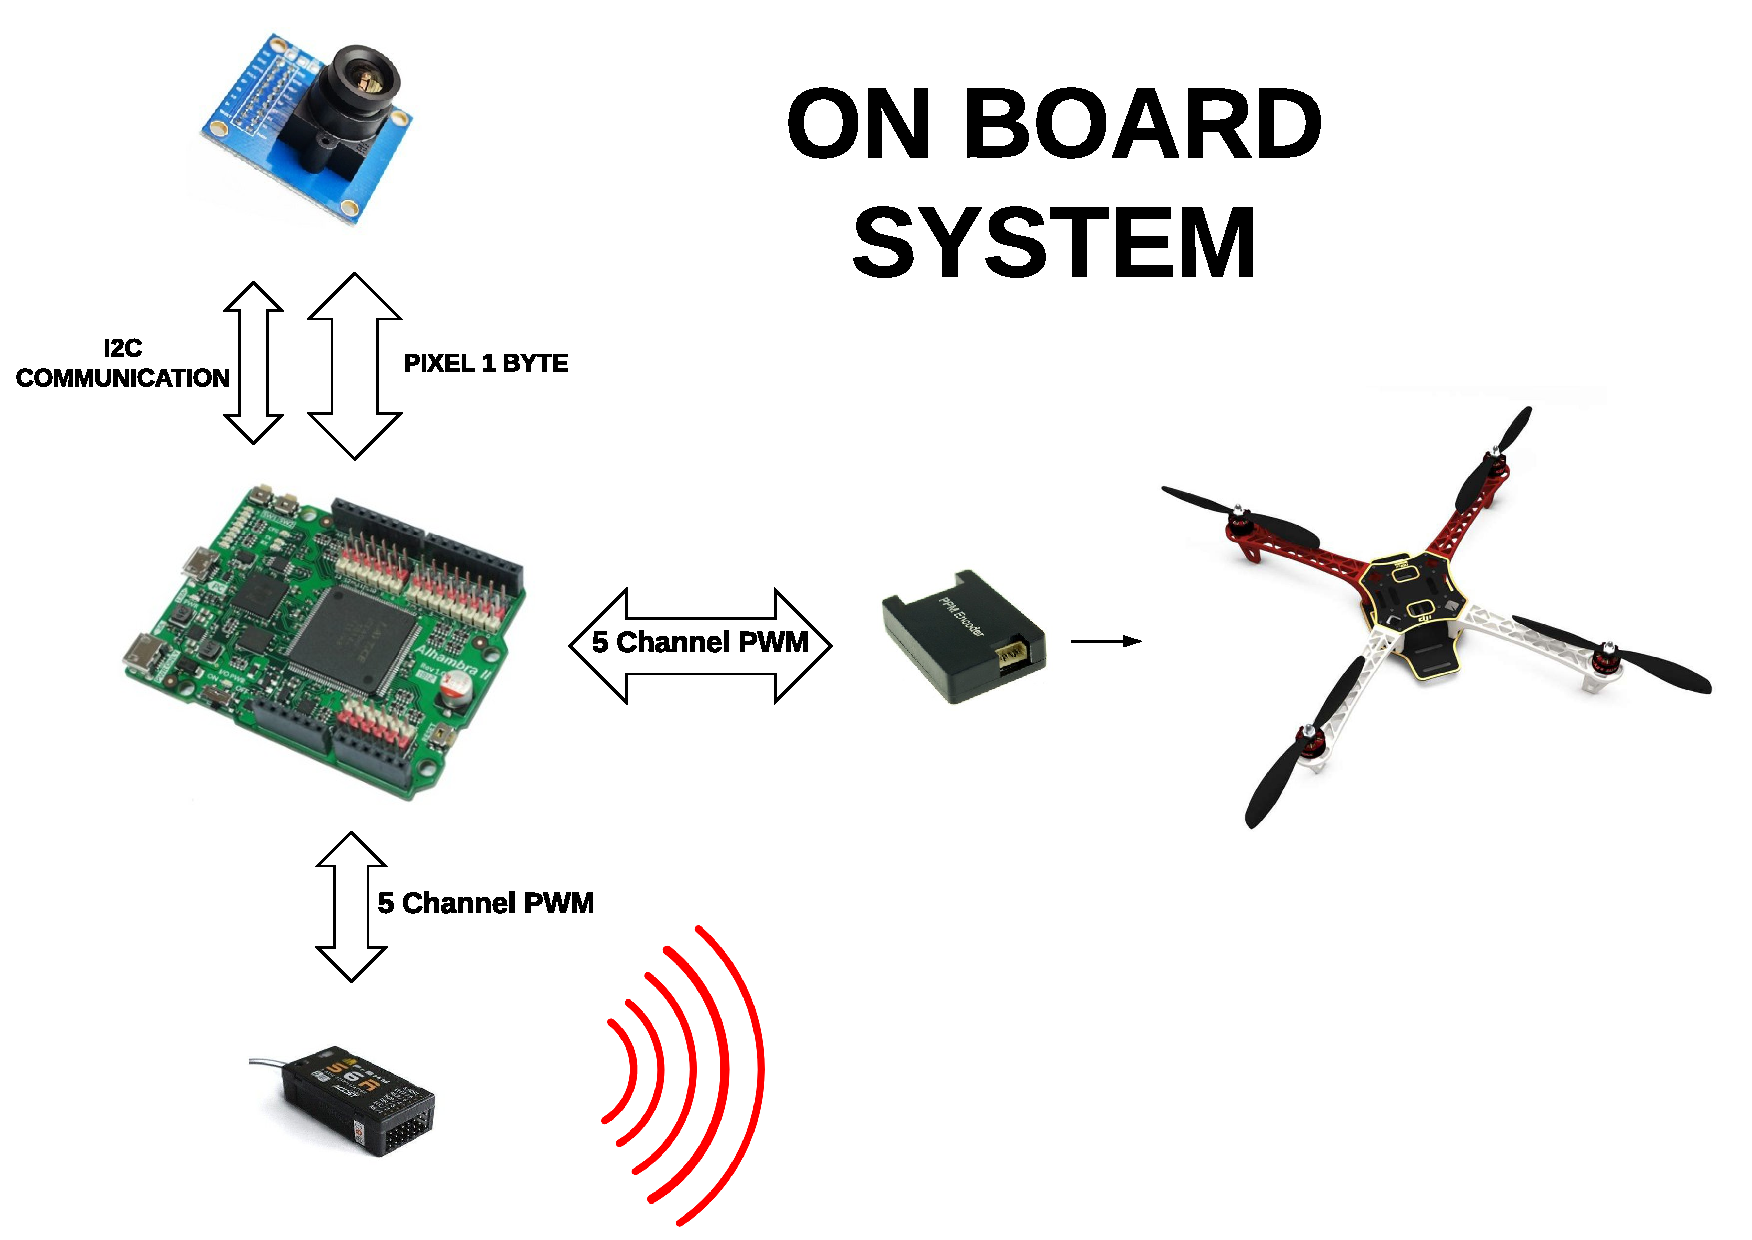
\includegraphics[trim = 0mm 0.5cm 0mm 0.5cm, clip,scale=0.38]{imagenes/Cuadricoptero_vision/on_board.pdf}
\end{figure}
\end{frame}


\subsection{Implementación de la percepción}

\begin{frame}{OV7670}
\begin{figure}[H]
	\center
	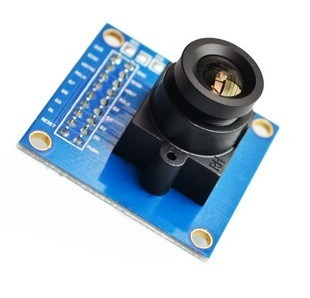
\includegraphics[scale=0.2, angle=0]{imagenes/Cuadricoptero_vision/OV7670}
\end{figure}
\begin{block}{}
	\begin{itemize}
		\item Transmisión de píxeles mediante 8 bits en paralelo
		\item Comunicación I2C para la configuración necesaria, 640x480, RGB565, frecuencia de píxeles.
	\end{itemize}
\end{block}
\begin{alertblock}{}
		\centering \textbf{NECESIDAD DE PROTOCOLO I2C} \pause
\end{alertblock}
\end{frame}

\begin{frame}{Protocolo I2C}
\begin{figure}[H]
	\center
	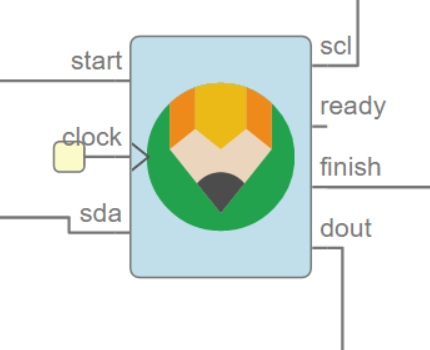
\includegraphics[scale=0.4, angle=0]{imagenes/Cuadricoptero_vision/I2C_write.PNG}
\end{figure}
\end{frame}

\begin{frame}{Protocolo I2C}
	\begin{figure}[H]
		\center
		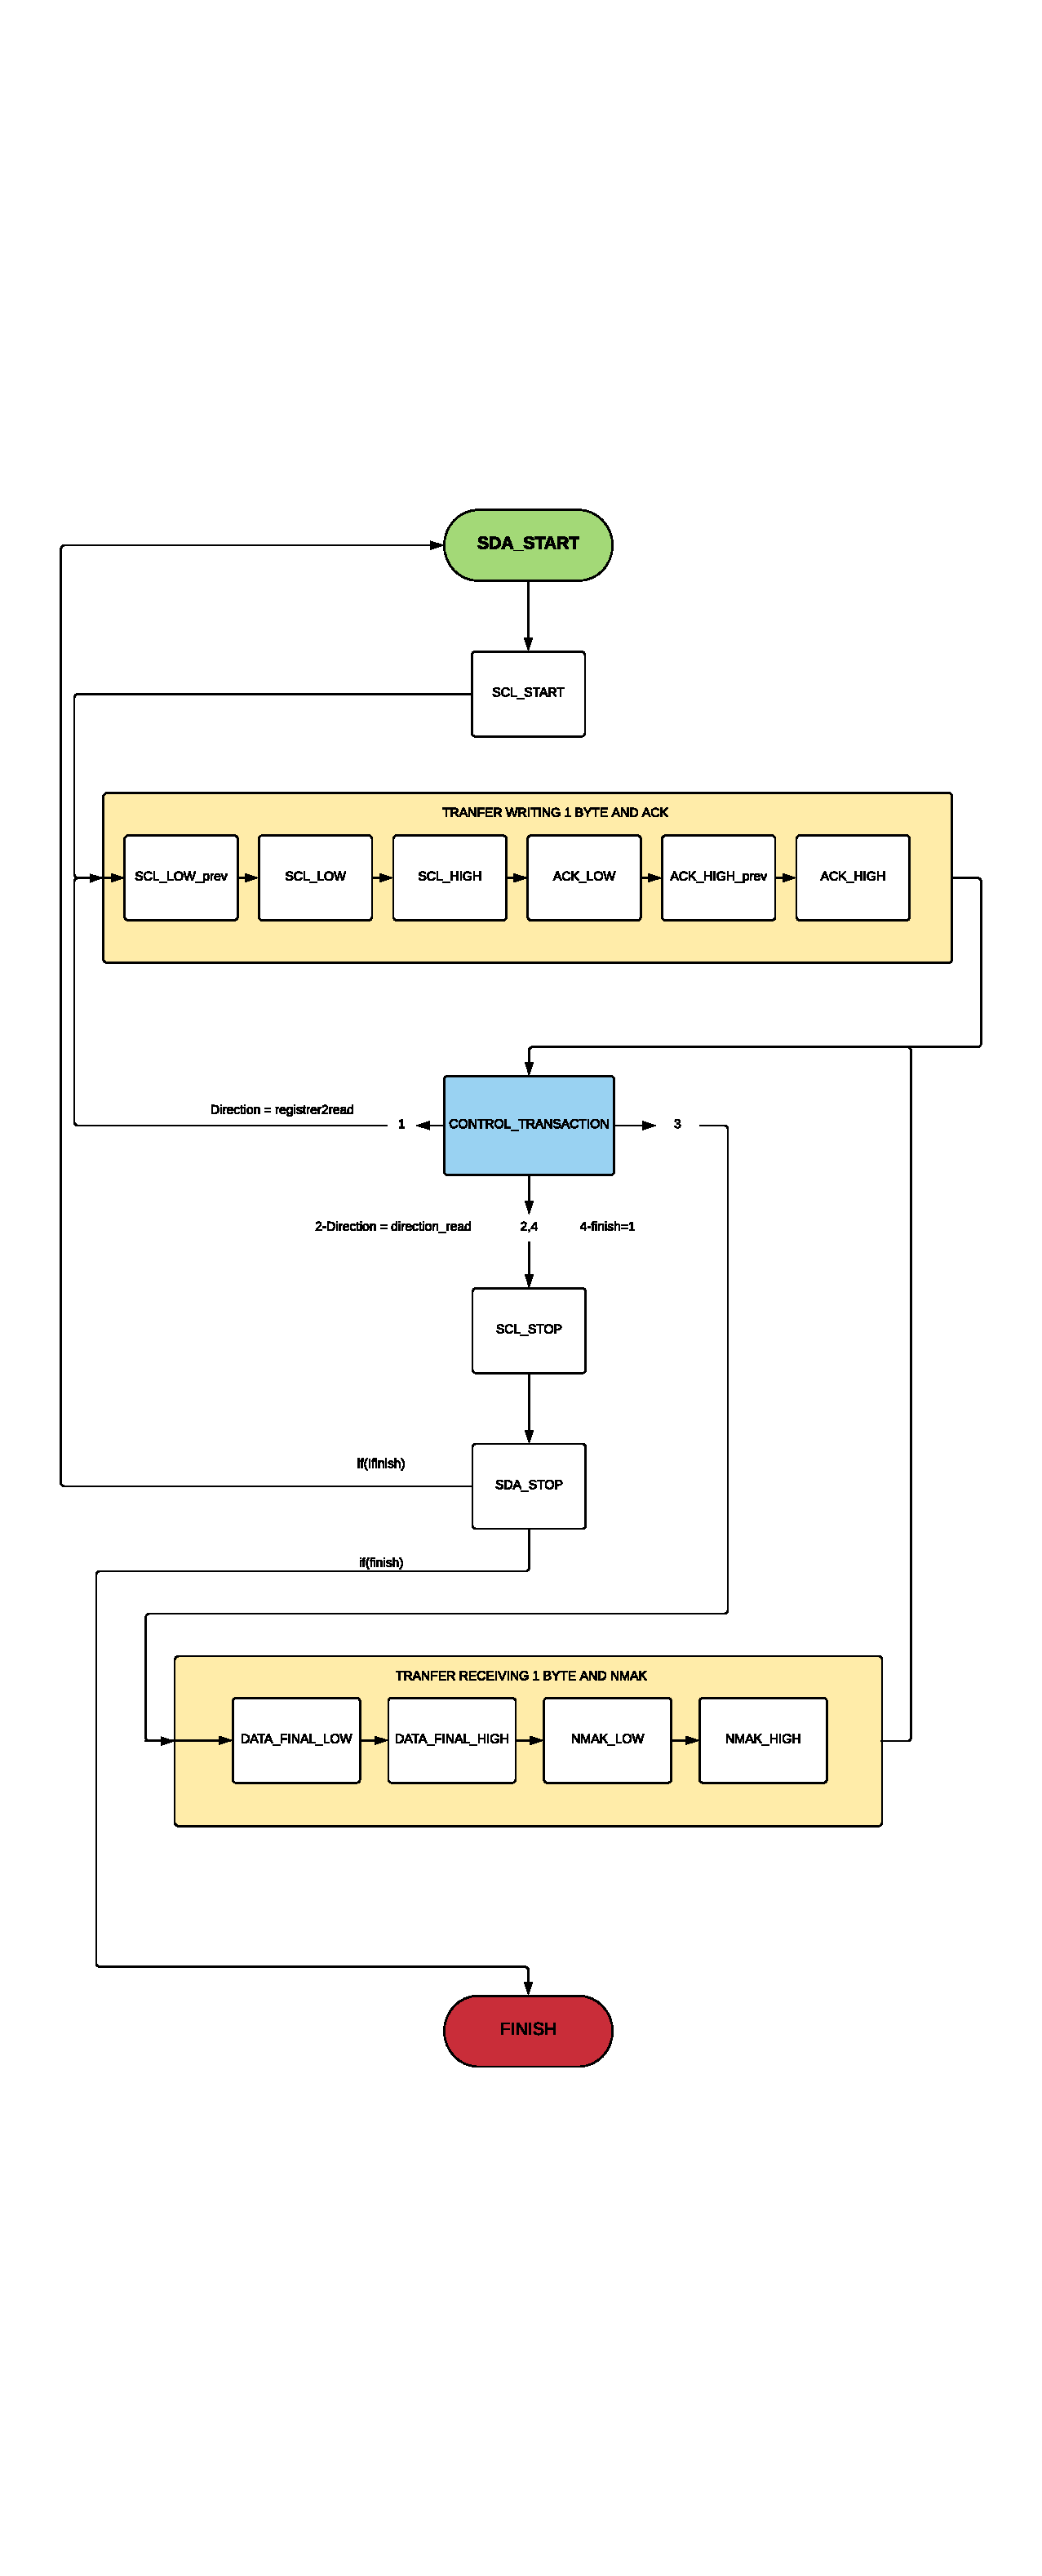
\includegraphics[trim = 0mm 8cm 0mm 10cm, clip,scale=0.23]{imagenes/Cuadricoptero_vision/I2C_WRITE.pdf}
	\end{figure}
\end{frame}

\begin{frame}{Reconocimiento del volumen y posición}
\begin{alertblock}{}
		\begin{equation*} 
	Volumen = Num_{\textup{pixeles filtrados}}/Num_{\textup{pixeles totales}}
	\end{equation*}
\end{alertblock}
\end{frame}

\begin{frame}{Reconocimiento del volumen y posición}
\begin{alertblock}{}
		\begin{equation*}\label{equation:acumx}
	Acum_{X} = \sum\textup{columns of filtered pixels}
	\end{equation*}
	
	\begin{equation*}\label{equation:acumx2}
	X_{media} = \frac{Acum_{X}}{Num_{\textup{filtered pixels}}}
	\end{equation*}
	
	\begin{equation*}\label{equation:acumx3}
	Error_{X} = X_{average}- \frac{width}{2}
	\end{equation*}
\end{alertblock}
\end{frame}


\begin{frame}{Reconocimiento del volumen y posición}
\begin{alertblock}{}
	\begin{equation*}\label{equation:acumy}
	Acum_{Y} = \sum\textup{row filtered pixels}
	\end{equation*}

	\begin{equation*}\label{equation:acumy2}
	Y_{average} = \frac{Acum_{Y}}{Num_{\textup{filtered pixels}}}
	\end{equation*}

	\begin{equation*}\label{equation:acumy3}
	Error_{Y} = Y_{average}- \frac{height}{2}
	\end{equation*}
\end{alertblock}
\end{frame}


\subsection{Diseño del control}
\begin{frame}{Diseño del control}
\begin{figure}[H]
	\center
	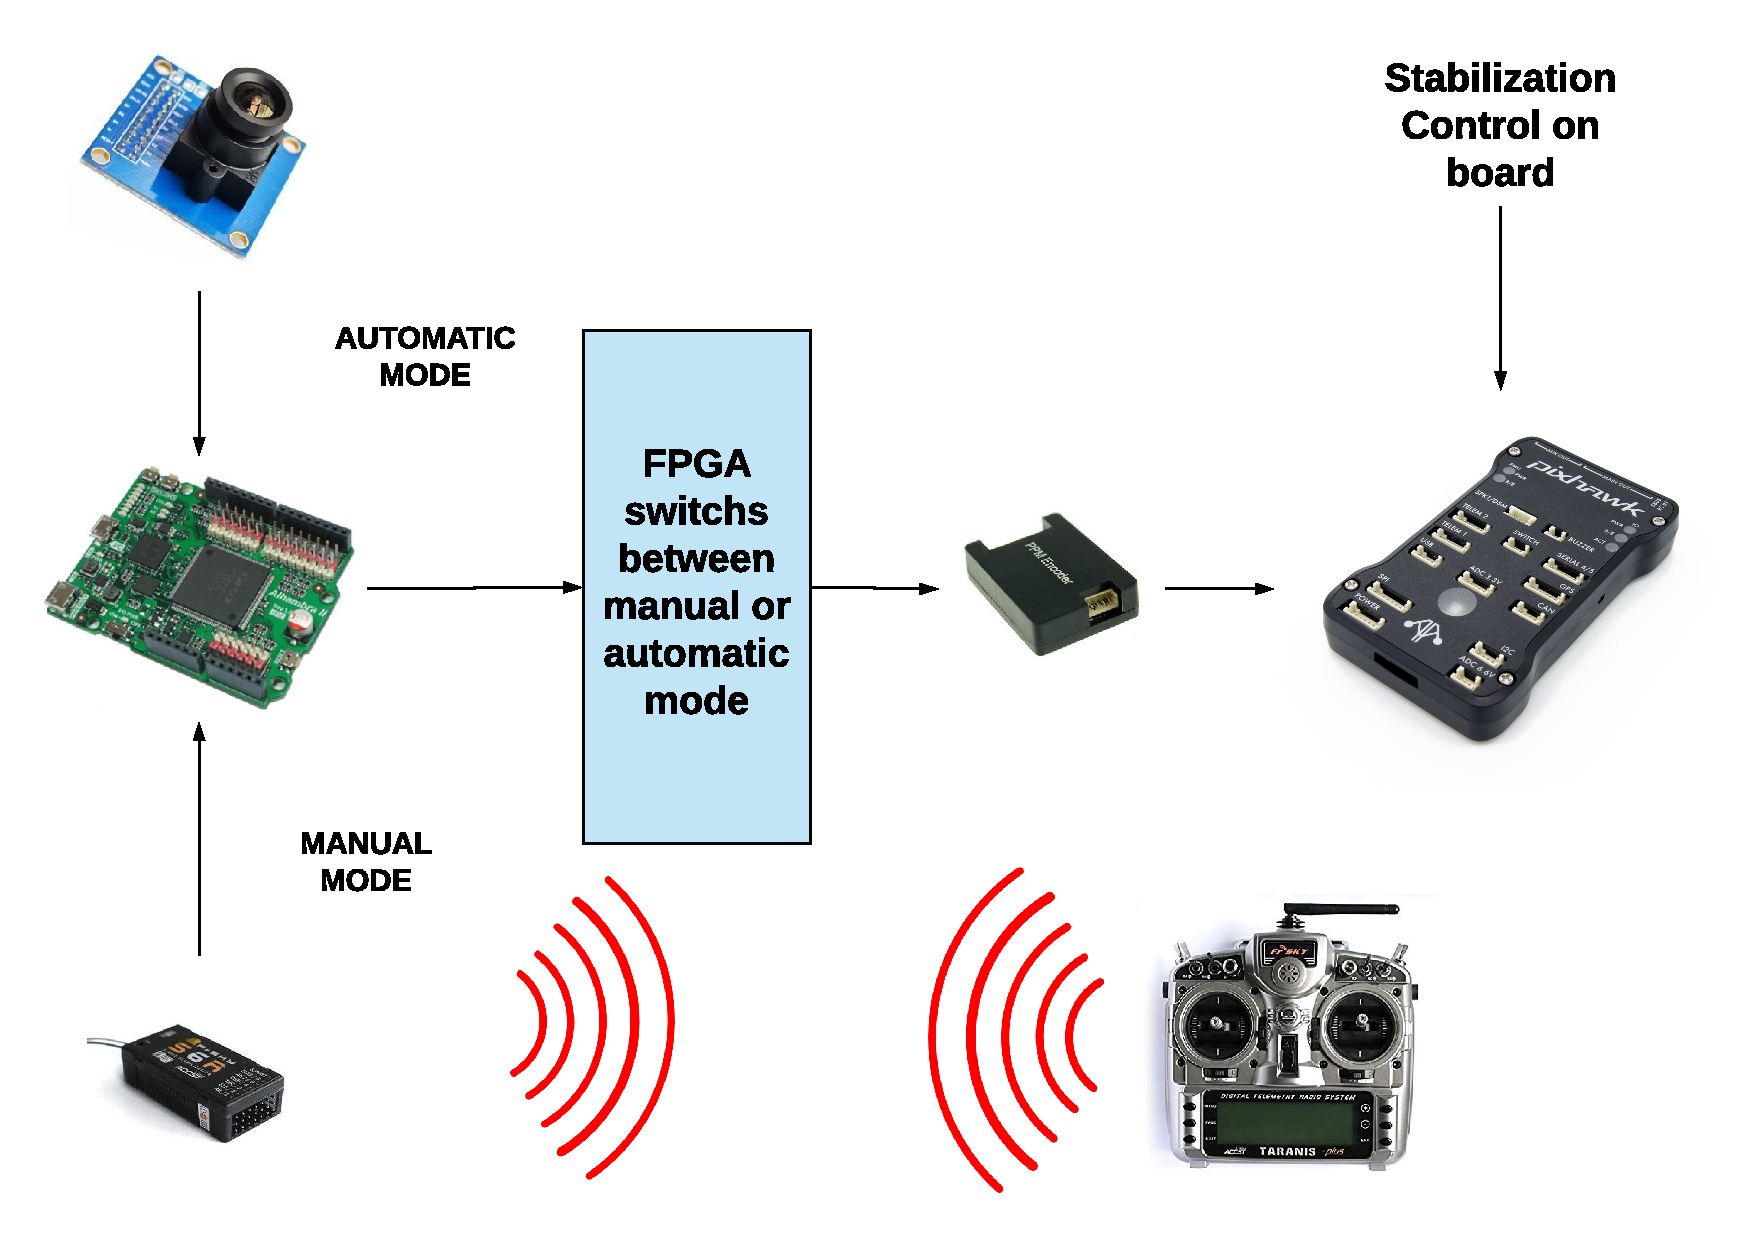
\includegraphics[trim = 0mm 0cm 0mm 0cm, clip,scale=0.39]{imagenes/Cuadricoptero_vision/control_implementation.pdf}
\end{figure}
\end{frame}
\section{Conclusiones y trabajo futuro}
\begin{frame}{Conclusiones}
Conclusiones de este trabajo
\end{frame}
\begin{frame}{Trabajo futuro}
\begin{block}{}
	\begin{itemize}
		\item Mejora de la mecánica del robot balancín \pause
		\item Integrar una mejora del control PD \pause
		\item Permitir fallos en el protocolo i2c \pause
		\item Permitir una comunicación bidireccional en microcontrolador-FPGA \pause
		\item Implementación del control a bordo del cuadricóptero 
	\end{itemize}
\end{block}
\end{frame}
\end{document}


